% プロジェクト学習中間報告書書式テンプレート ver.1.0 (iso-2022-jp)

% 両面印刷する場合は `openany' を削除する
\documentclass[11pt,a4paper,oneside]{jsbook}

\usepackage{bm}
\usepackage{float}
\usepackage{amsmath}
\usepackage{amsfonts}
\usepackage{amssymb}
\usepackage{blindtext}
\usepackage{here}
\usepackage[sectionbib]{chapterbib}
\usepackage[dvipdfmx]{graphicx}
\usepackage{funpro}
\usepackage{listings}

\setcounter{chapter}{1}
\setcounter{section}{0}

\thisYear{2018}
\jProjectName{ディーラーをやっつけろ! 複雑系の数理とシミュレーション}
\eProjectName{Beat the dealer! Mathematics of Complex Systems and Simulation.}
\ProjectNumber{3}
\jGroupName{グループ~1}
\eGroupName{Group~1}
\ProjectLeader{1014207}{菱田美紗紀}{Misaki~Hishida}
\GroupLeader  {1016123}{薩田凱斗}{Kaito~Satta}
\SumOfMembers{9}
\GroupMember  {1}{1016007}{柏田輝}{Hikaru~Kashiwada}
\GroupMember  {2}{1016042}{尾崎拓海}{Takumi~Ozaki}
\GroupMember  {3}{1016078}{伊藤晋之介}{Shinnosuke~Ito}
\GroupMember  {4}{1016087}{轟木文弥}{Fumiya~Todoroki}
\GroupMember  {5}{1016118}{葛西隼人}{Hayato~Kasai}
\GroupMember  {6}{1016175}{柿崎大輝}{Daiki~Kakizaki}
\GroupMember  {7}{1016184}{鳥谷航大}{Koudai~Toriya}
\GroupMember  {8}{1016207}{渡邊凛}{Rin~Watanabe}
\GroupMember  {9}{1016231}{米村祥裕}{Yoshihiro~Yonemura}
\jadvisor{川越敏司,川口聡,斎藤朝輝}
\eadvisor{Toshiji~Kawagoe,Satoshi~Kawaguchi,Asaki~Saitou}
\jdate{2018年7月22日}
\edate{July~22, 2018}

\renewcommand{\thesection}{\arabic{chapter}.\arabic{section}}%

% 画像ファイル (EPS, EPDF, PNG) を読み込むために
\usepackage[dvipdfmx]{graphicx,color}
\pagestyle{empty}
\advance\textheight\headheight \headheight=0pt
\advance\textheight\headsep    \headsep=0pt
\advance\textheight\footskip   \footskip=0pt
\textheight=738truept
\advance\textwidth\marginparsep \marginparsep=0pt
\advance\textwidth\marginparwidth \marginparwidth=0pt
\advance\textwidth\oddsidemargin \oddsidemargin=0pt
\evensidemargin=\oddsidemargin
\textwidth=50zw
\advance\textwidth2zw
\columnsep=2zw
\topmargin=-5.4mm
\oddsidemargin=-7.4mm

\begin{document}
\maketitle
\pagenumbering{roman}
\fontsize{10}{18}\selectfont
%前付け
\frontmatter

% 和文概要
\begin{jabstract} 
\ \ 本プロジェクトでは、カジノにおいて最もポピュラーなゲームの一つであるブラックジャックを取り扱っている。
ブラックジャックに関する代表的な行動戦略としてベーシックストラテジー、カウンティングというものがある。これ
らはプレイヤーの期待利得を増大させプレイヤーにとって有利な状況を作り出した。しかしカジノ側の対策によって、
戦略を単純に採用し実行することは困難になり、期待利得も減少することになった。そこで我々は既存の戦略と比較して
 3つの観点から優れた戦略を見つけ出すことを試みた。1つ目はプレイヤーの利得を既存の戦略に比べて増加させること、
 2つ目はカジノ側の対策を回避することである。3つ目はプレイヤーが覚えやすく、実行可能なものであることである。\\

\ \ 戦略を見つけるにあたって、現在までに我々は既存の戦略として最も有名なベーシックストラテジーと呼ばれる戦略
についてどの程度確からしく、単純に考えられる他の手法に比べてどの程度プレイヤーに有利なのかを検証した。ブラック
ジャックのシミュレータを作成し、を行った。その勝率により戦略の優劣を比較した。このとき、戦略の複雑性を考
慮するとベーシックストラテジーは改善の余地があるという結果が得られた。
% 和文キーワード
\begin{jkeyword}
カジノ,\ ブラックジャック,\ ベーシックストラテジー,\ 複雑性
\end{jkeyword}
\bunseki{※轟木文弥}
\end{jabstract}

%英語の概要
\begin{eabstract} 
\ \ In this project, we deal with Blackjack, one of the most popular games in the casino. There are
also basic strategies and counting as representative behavior strategies concerning blackjack. This
has increased the player's expectation gain and created a situation that is also true for the player.
 It is difficult to easily adopt and execute the strategy by the casino side measures, and the expected
  value has also been reduced. Then, we tried trying to find a winning strategy from three perspectives 
  compared to existing strategy: one to increase the gain of the target player compared to the existing 
  strategy, two to casino side The third is to make it easy for players to memorize and execute.\\
\ \ In finding a strategy, we have verified to what extent the strategy called the basic strategy which 
is most familiar as an existing strategy is confirmed up to now and to what extent it is advantageous to 
the player compared with other methods which can simply be considered. We made a blackjack simulator and 
played a game. Based on the winning percentage, we compared the merits of strategies. At this time, considering 
the complexity of the strategy, the result that the basic strategy has room for improvement was obtained.
% 英文キーワード
\begin{ekeyword}
casino, blackjack, basic strategies, complexity
\end{ekeyword}
\bunseki{※轟木文弥}
\end{eabstract}

\tableofcontents
\newpage

\pagenumbering{arabic}

\chapter{研究背景}
%ソースが不明なのでとりあえず暫定削除
%\section{ブラックジャックの概要と歴史}
%ブラックジャックのルーツは1570年にさかのぼる。このころはまだ「ブラックジャック」という名称は使われていなかった。1875年に出版された「The American Hoyle of 1875」という書籍で「ブラックジャック」として紹介されたのが初出である。このゲームが考え出された当初は金銭を賭けることはなく、身内内で楽しむだけのゲームであった。
%はじめて金銭が賭けられるようになったのは1910年頃のアメリカ、インディアナ州であるといわれている。当時は競馬以外のギャンブルが違法であり、ブラックジャックも違法カジノでのみ行われていた。その後インディアナ州以外のアメリカ全土に広がっていった。そして現在世界中のカジノで合法的に楽しまれるポピュラーなゲームになった。
%\bunseki{※菱田美紗紀}

\section{ブラックジャックの戦略の歴史}
斎藤(1999)によれば、ブラックジャックの戦略については1950年にメリーランド州のとある米国陸軍の研究所に所属していたRoger、Nash、Baldwinらが研究したものが始まりであるといわれている。その後計算機の性能向上より、ブラックジャックのシミュレーションが容易になったことでさらに戦略の研究は進んでいった。
ブラックジャックには主に有名な戦略が2つ存在する。

1つ目がベーシックストラテジーと呼ばれる戦略だ。ベーシックストラテジーはディーラーのアップカードと自分の手札の状況によってプレイヤーが選択するべき最適な行動を決定するという戦略である。

2つ目はカウンティングと呼ばれる戦略だ。カウンティングはブラックジャックのゲーム中で既に使われたカードを記憶することで、プレイヤーが有利になるように戦略を決定していくというものである。

前期ではベーシックストラテジーについて調査をした。カウンティングについては後期に詳しく調査していく予定である。
なお、カウンティングはカジノ側に対策をされており、この戦略を使用していることがカジノ側に気づかれた場合、プレイヤーはカジノから退場させられることもある。
\bunseki{※伊藤晋之介}
\chapter{課題解決のプロセス}
\section{ルール}
\subsection{ブラックジャック}
ブラックジャックとは、トランプを使用したゲームで、カジノで行われる有名なギャンブルの一つである。ブラックジャックはプレイヤーとディーラー(カジノ側のプレイヤー)が戦うゲームで、勝敗はトランプの合計で決まり、合計が21以下で相手より大きい方の勝利である。また、ブラックジャックを極めることが出来れば全てのカジノで勝ち易くなると言われており、カジノでの勝率を上げる手段としても注目されている。

\subsection{ブラックジャックのルール}
トランプの扱いについて
\begin{itemize}
\item ジョーカーは扱わない
\item トランプのマークは関係がない
\item 数字は2~9まではそのままの数
\item 10・J・Q・Kは10として扱う
\item Aは11または1で都合の良いほうとして扱う
\end{itemize}
勝敗条件
\begin{itemize}
\item 相手よりも合計が大きく、22より小さい方が勝ち
\item 22以上であるとバーストといい、バーストした側の負けとなる
\item 合計が同じ場合は引き分けとなる
\item プレイヤーとディーラーの両方がバーストの場合、ディーラーの勝ちとなる
\item 2枚の手札で合計が21になるとナチュラルブラックジャックといい、3枚以上の合計21と対決した場合、ナチュラルブラックジャックの方が勝ちになる
\end{itemize}
賭け金の扱い
\begin{itemize}
\item プレイヤーが普通に勝つと賭け金の2倍が払い戻される
\item プレイヤーがナチュラルブラックジャックで勝つと賭け金の2.5倍が払い戻される
\item ディーラーが勝つと賭け金を没収される
\end{itemize}
プレイヤーの選択肢
\begin{itemize}
\item ヒット:カードを1枚追加すること、何度でもできる
\item スタンド:カードを引かずに今のカードで勝負すること
\item サレンダー:負けを認めて、賭け金の半分をもらうことができる。最初の行動でのみ使える。
\item ダブルダウン:賭け金を2倍にし、1度だけヒットをする。最初の行動でのみ使える。
\item スプリット:最初のカード2枚が同じ数字だった場合使用可能。最初の賭け金と同じ金額を追加して、それを2つに分割して、それぞれで勝負することができる
\item インシュランス:ディーラーの表向きのカード(アップカード)が「A」の場合使える。最初の賭け金の半分を使い、ディーラーがナチュラルブラックジャックになればその賭け金の2倍が払い戻される。
\item イーブンマネー:自分の手札がナチュラルブラックジャックである場合に行うインシュランスのこと。このイーブンマネーの場合は元の賭金の半額をわざわざテーブルに出す必要はなく、ただ単にイーブンマネーと声を出して宣言するだけでよい。宣言するとすぐその場でディーラーは元の賭金と同じ額だけ支払ってくれる。なぜならディーラーにブラックジャックが完成していようがいまいが結果は必ず同じになるからだ。もしディーラーにブラックジャックが完成していた場合、インシュランスとして掛けた保険料の倍の金額が支払われ、もともとの勝負の方はお互いブラックジャックなので引き分け。結果として保険金だけを受け取ることになる。逆にもしディーラーにブラックジャックができていなかった場合、当然保険料は没収されるが、一方ゲームそのものの勝負はプレイヤー側の勝ちとなり賭金の1.5倍の勝ち金を受けることになる。つまり結果として差し引き 「賭金と同じ額だけの儲け」 ということになる。以上のようにイーブンマネー保険を掛けた場合はディーラーの見えていない方のカードに関係なく自動的に賭金の1倍の勝ちが確定することになる。よってイーブンマネーの場合はイーブンマネーと宣言するだけで良い。
\end{itemize}

\subsection{ディーラーの行動}
プレイヤーに比べ、ディーラーが選択できる行動は少なく、ヒットとスタンドしかできない。その上、ディーラーの行動はあるルールが存在する。そのルールとは「ディーラーは17以上になるまでヒットを続けなければならない」というルールだ。これによりディーラーの最終合計は17,18,19,20,21,バーストのどれかになる。

\subsection{ゲームの流れ}
まず山札をシャッフルし、カットカードと呼ばれるカードを山札にランダムに入れる。カーットカードは、ゲームが終わりを示すカードである。その後ゲームが始まり、まず賭け金を出す。その後、プレイヤー、ディーラーの順にカードが1枚配られ、再度同じように2枚目が配られます。このときプレイヤーのカードは2枚とも表向きですがディーラーは1枚を表向き(アップカード)でもう1枚は裏向き(ダウンカード)です。カードが配り終えると、プレイヤーの行動です。プレイヤーがバースト、もしくはスタンドした場合、プレイヤーの行動は終了である。次はディーラーの行動です。ディーラーがスタンド、もしくはバーストした場合、ディーラーの行動は終了である。ここで勝敗を確認し、それに応じた支払いが行われて、ゲームが終了する。
    \section{ブラックジャックにおける従来の戦略}
    \subsection{従来の戦略}

        ブラックジャックにおける主な既存の戦略はベーシックストラテジーとカウンティングである。

        ベーシックストラテジーは一回ごとのゲームを想定しており、自分の手札とアップカードのみによって勝率が高い行動を決定する戦略である。そのため、行動を決定するまでに使用されたカードは行動決定に影響せず、残りのカードの予測も行わない。

        また、カウンティングは、デックをシャッフルしない状態で、カードを使い続けた場合のゲームに対して発生する利得を最大にすることを目的とした戦略である。ゲームで使われたカードを記憶し、残りのカードを予測する。そこから自分の有利・不利を決定し賭け金の増減を行うという戦略である。
        \bunseki{※鳥谷航大}
    \subsection{ベーシックストラテジー}
        ブラックジャックの最も有名な既存の戦略としてベーシックストラテジーという戦略が挙げられる。ベーシックストラテジーは1962年にEdward Thorp氏の書籍『Beat The Dealer: A Winning Strategy for the Game of Twenty One』にて発表された戦略である。元となるアイデアとして、Roger Baldwinらが1956年に発表した「The Optimum Strategy in Blackjack」が使用されている。
        \bunseki{※鳥谷航大}
    \subsection{ベーシックストラテジーの導出}
        ベーシックストラテジーは以下の前提条件を持つ。
        \begin{itemize}
            \item 前提条件\\
                使用されているデック数は無限である
        \end{itemize}

        つまり、場にカードが何枚使われていても、どのカードを引く確率も常に13分の1であるとし、この前提条件の元で、アップカードと手札の合計値からヒットした時とスタンドした時の勝率から導出される。具体的には以下のような手順によって導出する。
        \begin{enumerate}
            \item プレイヤーの手札の合計値とアップカードの組み合わせごとにヒットした場合の勝率とスタンドした場合の勝率を求める
            \item ヒットした場合の勝率からスタンドした場合の勝率を引き、その差を求める
            \item 求めた差が0以上であった場合はヒット、0未満であった場合はスタンドが有効であるとする
        \end{enumerate}

        ベーシックストラテジーの導出に移る前に以下のような定義を行う。
        \begin{itemize}
            \item[] x: プレイヤーに最初に配られた2枚のカードの合計値 \((x < 21)\)
            \item[] D: アップカード
            \item[] M(D): ディーラーのアップカードによるプレイヤーがスタンドできる最低の手札の合計値
            \item[] J: プレイヤーが1回ヒットした後の最終的な手札の合計値
            \item[] T: ディーラーの最終的な手札の合計値 (\(T \geq 17\))
            \item[] \(E_{d,x}\): プレイヤーの手札の合計値がxの時にヒットした場合の勝率
            \item[] \(E_{s,x}\): プレイヤーの手札の合計値がxの時にスタンドした場合の勝率
            \item[] \(P(Y)\): 式Yが成立する確率
        \end{itemize}

        まず\(E_{s,x}\)について考える。\(E_{s,x}\)とはプレイヤーの手札の合計値が$x$である時にスタンドした場合の勝率である。つまり、\(T > 21 \)または\(T < x\)の時、プレイヤーは$x$でスタンドした場合、そのゲームに勝利し、\(x < T \leq 21\)の時、プレイヤーはxでスタンドした場合、そのゲームに敗北する。また、\(T = x\)の時は引き分けとなり、$x$でスタンドした場合利得は0である。これらのことから\(E_{s,x}\)は以下のような式によって表せる。
        \begin{displaymath}
            \begin{split}
                E_{s,x} = &P(T > 21) + P(T < x) - P(x < T \leq 21)\\
                &= 2P(T > 21) + 2P(T < x) + P(T = x) - 1
            \end{split}
        \end{displaymath}
        
        次に\(E_{d,x}\)について考える。\(E_{d,x}\)とはプレイヤーの手札の合計値が$x$である時にヒットした場合の勝率である。手札の合計値が$x$でヒットした場合は以下の3つの場合に分けられる。
        \begin{enumerate}
            \item \(J < 17\)\\
                Tは常に17以上であるから、この時にプレイヤーが勝利する期待値は以下のように表せる。
                $$P(T > 21) - (1 - P(T > 21)) = 2P(T > 21) - 1$$
            \item \(17 \leq J \leq 21\)\\
                同様にこの時にプレイヤーが勝利する期待値は、
                $$P(T > 21) + P(T < J) - P(J < T \leq 21)$$
                となる。
            \item \(J > 21\)\\
                この時、Tがどのような値でもプレイヤーは敗北する。つまり期待値は-1となる。
        \end{enumerate}

        以上のことから\(E_{d,x}\)は、
        \begin{displaymath}
            \begin{split}
                E_{d,x} = &P(J < 17)(2P(T > 21) - 1) - P(J > 21)\\
                &+ \sum_{j=17}^{21}P(J = j)(P(T > 21) + P(T < j) - P(j < T \leq 21))
            \end{split}
        \end{displaymath}
        となる。
        ここで\(E_{d,x}\)の第3項の部分に注目する。第3項は、Tは常に17以上\((T \leq 17)\)であること、Jは17以上21以下\((17 \leq J \leq 21)\)であることから以下のような変形を行うことができる。
        \begin{displaymath}
            \begin{split}
                \sum_{j=17}^{21}&P(J = j)(P(T > 21) + P(T < j) - P(j < T \leq 21)\\
                &= \sum_{j=17}^{21}P(J = j)(P(T > 21) + P(T < j) - (1 - P(T > 21) - P(T < j) - P(T = j))\\
                &= \sum_{j=17(}^{21}P(J = j)(2P(T > 21) - 1 + 2P(T < j) + P(T = j))\\
                &= (2P(T > 21) - 1)\sum_{j=17(}^{21}P(J = j) + 2\sum_{j=17(}^{21}P(J = j)P(T < j) + \sum_{j=17(}^{21}P(J = j)P(T = j)\\
                &= (2P(T > 21) - 1)\sum_{j=17(}^{21}P(J = j) + 2P(T < J \leq 21) + P(T = J \leq 21)\\
            \end{split}
        \end{displaymath}

        また、\(P(J < 17)\) + \(\sum_{j=17}^{21}P(J = j) = P( J \leq 21)\)と書けるため、\(E_{d,x}\)は、
        \begin{displaymath}
            \begin{split}
                E_{d,x} &= P(J < 17)(2P(T > 21) - 1) - P(J > 21)\\
                        &\quad+ (2P(T > 21) - 1)\sum_{j=17(}^{21}P(J = j) + 2P(T < J \leq 21) + P(T = J \leq 21)\\
                        &= (2P(T > 21) - 1)(P(J < 17) + \sum_{j=17}^{21}P(J = j)) - P(J > 21)+ 2P(T < J \leq 21) + P(T = J \leq 21)\\
                        &= (2P(T > 21) - 1)P(J \leq 21) - P(J > 21) + 2P(T < J \leq 21) + P(T = J \leq 21)\\
                        &= (2P(T > 21) -1)(1 - P(J > 21)) - P(J > 21) + 2P(T < J \leq 21) + P(T = H \leq 21)\\
            \end{split}
        \end{displaymath}
        となる。したがって、行動決定式\(E_{d,x} - E_{s,x}\)は、
        \begin{displaymath}
            \begin{split}
                E_{d,x} - E_{s,x} &= (2P(T > 21) -1)(1 - P(J > 21)) - P(J > 21) + 2P(T < J \leq 21) + P(T = H \leq 21)\\
                &\quad- ( 2P(T > 21) + 2P(T < x) + P(T = x) - 1)\\
                &= -2P(T < x) - P(T = x) -2P(T > 21)P(J > 21) + 2P(T < J \leq 21) + P(T = J \leq 21)\\
            \end{split}
        \end{displaymath}
        となる。
        %\bunseki{※鳥谷航大}
    %\subsection{ベーシックストラテジーの導出}
        ベーシックストラテジーの導出を行う上で、$x$について以下の3つの場合分けを行う。
        \begin{eqnarray}
            x<12\\
            12 \leq x\leq 16\\
            x>16
        \end{eqnarray}
        \subsubsection{}
            $x<12$のとき、$T \geq 17$であるから、$P(T < x)$と$P(T = x)$は0である。同様に、$P(J > 21)$も0であるから、$E_{d,x} - E_{s,x}$は常に0以上($E_{d,x} - E_{s,x} \geq 0$)となる。よって$x < 12$において、プレイヤーの行動は全てヒットとなる。
        \subsubsection{}
            $12\leq x \leq 16$のとき、1.4.1と同様に$P(T < x)$と$P(T = x)$は0である。この時の行動決定式$E_{d,x} - E_{s,x}$は以下のように書ける。
            \begin{displaymath}
                E_{d,x} - E_{s,x} = -2P(T>21)P(J>21) + \sum_{t-17}^{21}P(T=t)(2P(t<J\leq21) + P(J=t))
            \end{displaymath}
            また、プレイヤーが引いてくるカードの確率は全て同じであるため、
            \begin{eqnarray}
                \begin{split}
                    &P(J-x=10)=4/13 \notag\\
                    &P(J-x=i)=1/13 \quad i=2,3,...,9,(1,11) \notag
                \end{split}
            \end{eqnarray}
            と考えられる。したがって、
            \begin{displaymath}
                \begin{split}
                    &P(J>21)=\frac{1}{13}(x-8)\\
                    &P(T<J\leq21)=\frac{1}{13}(21-T)\\
                    &P(J=T)=\frac{1}{13}\\
                \end{split}
            \end{displaymath}
                とそれぞれ表すことができるため、$E_{d,x} - E_{s,x}$は以下のように書ける。
            \begin{displaymath}
                E_{d,x} - E_{s,x} = -\frac{2}{13}(x-8)P(T>21)+\frac{1}{13}\sum_{t-17}^{21}P(T=t)(43-2t)
            \end{displaymath}
            ここで$x=x_0$として、$E_{d,x_0} - E_{s,x_0}=0$の時を考える。この時、$x_0$は、
            \begin{displaymath}
                \begin{split}
                    x_0&=8+\frac{1}{2}\frac{\sum_{t=17}^{21}(43-2t)P(T=t)}{P(T>21)}\\
                \end{split}
            \end{displaymath}
            となる。このことから、$12\leq x\leq 16$のとき、$M(D)=[x_0]+1$となる。
        \subsubsection{}
            $x>16$のとき、まず、$x=17$を考える。この時$E_{d,x}-E_{s,x}$は、
            \begin{displaymath}
                \begin{split}
                    E_{d,x}-E_{s,x}=-\frac{18}{13}P(T>21)-\frac{5}{13}P(T=17)+\frac{1}{13}\sum_{t=18}^21(43-2t)P(T=t)
                \end{split}
            \end{displaymath}
            となる。この時$E_{d,x}-E_{s,x}$は、全ての$D$に対して常に0未満となる。つまり、$E_{d,x}-E_{s,x}<0$であるから、$M(D)\leq 16$となる。
        
        以上のことから、ベーシックストラテジーは表\ref{basicstrategytable}となる。この戦略表は、縦軸がプレイヤーの手札の合計値を表し、横軸がディーラーのアップカードを表す。それぞれの交わる場所がプレイヤーの取る最適な行動となっていて、Sがスタンド、Hがヒットを表す。例えば、プレイヤーの手札の合計値が12、ディーラーのアップカードが2であった場合、プレイヤーの取るべき行動はH、つまりヒットとなる。
        \begin{table}[H]
            \begin{center}
            \label{basicstrategytable}
            \caption{ベーシックストラテジーの戦略表}
            \begin{tabular}{|c|c|c|c|c|c|c|c|c|c|c|}
            \hline
                        & \multicolumn{10}{c|}{ディーラーのアップカード}     \\ \hline
            プレイヤーの手札の合計 & 2 & 3 & 4 & 5 & 6 & 7 & 8 & 9 & 10 & A \\ \hline
            19以上        & S & S & S & S & S & S & S & S & S  & S \\ \hline
            18          & S & S & S & S & S & S & S & S & S  & S \\ \hline
            17          & S & S & S & S & S & S & S & S & S  & S \\ \hline
            16          & S & S & S & S & S & H & H & H & H  & H \\ \hline
            15          & S & S & S & S & S & H & H & H & H  & H \\ \hline
            13,14       & S & S & S & S & S & H & H & H & H  & H \\ \hline
            12          & H & H & S & S & S & H & H & H & H  & H \\ \hline
            11以下        & H & H & H & H & H & H & H & H & H  & H \\ \hline
            \end{tabular}
            \end{center}
            \end{table}
        \bunseki{※鳥谷航大}
    

%既存戦略の検証に関する項目
\chapter{プロジェクトの目的}
本プロジェクトでは、3つの目標を設定した。
\begin{description}
\item[目標1] 最終的な勝率が5割以上になること
\begin{itemize}
\item{後述するが、シミュレーションを行った結果、ベーシックストラテジーを使用した際の勝率が4割程度しかなかった。そのためそれ以上の勝率が出せる戦略を発見するということを目標とした。また全体的な勝利数が勝ち越せるように5割以上とした。}
\end{itemize}
\item[目標2]人間が扱いやすいこと
\begin{itemize}
\item{人間が扱いやすいことについては独自の複雑性を定義し、複雑性と勝率の両方を考慮し一番効率が良いと考えられるものを探索することとした。}
\end{itemize}
\item[目標3]戦略を使用していることがカジノ側に検知されにくいこと
\begin{itemize}
\item{カジノ側がどのような基準でプレイヤーが戦略を使用していることを判断しているのかを理解することでカジノ側に検知されにくい戦略を作ることを目標とする。}
\end{itemize}
\end{description}
以上の3点を本プロジェクトの前期の目的とした。後期の目的については後期に設定する予定である。
\bunseki{※伊藤晋之介}

\chapter{ベーシックストラテジーの検証}
\section{従来の戦略の問題点}
まず、ベーシックストラテジーの問題点について述べる。この戦略はデック数が無限個を想定しており、すでに引いたカードの種類や枚数を考慮していない点である。
まず、基本的にカジノで行われるゲームではデック数は有限である。デック数が有限であるということは、以前に引いたカードの種類によって、次に引くカードの確率が変化していくということである。例えば、プレイヤーが2人、デック数が1のゲームをしていると仮定する。ディーラーのアップカードがハートのエース、プレイヤー1の初期の手札がダイヤのエースとクローバーのエース、プレイヤー2の初期の手札がスペードのエースとハートの2が配られたとする。この時点でデック内のエースのカードはすべて配られてしまい、以後のゲームでエースが出る確率は0になっている。しかし、デック数を無限に設定すると、以後のゲームでもエースは無限に存在することになり、確率は4/52になってしまう。これが、デック数無限のシミュレーションと実際のゲームの相違点である。このような相違点を考慮しないため、実際の勝率とは異なってしまい、利益についてもばらつきが出てしまうのである。
またこの戦略は勝率が4割程度しかなく、勝利数だけで言えばカジノ側に負けてしまう。
カウンティングの問題点については後期に詳しく調査する予定である。
\bunseki{※菱田美紗紀}

\section{戦略同士の比較}
Thorp氏によって考案されたベーシックストラテジーについて検証を行う.
ベーシックストラテジーの性能評価のために比較対象として6つの戦略を考えた.
比較対象となる戦略は次の通りである.

\begin{itemize}
  \item ベーシックストラテジー改変1
  \item ベーシックストラテジー改変2
  \item プレイヤーの合計値が15以上になるまでヒットする戦略
  \item プレイヤーの合計値が16以上になるまでヒットする戦略
  \item プレイヤーの合計値が17以上になるまでヒットする戦略
  \item プレイヤーの合計値が18以上になるまでヒットする戦略
\end{itemize}

以上の6つの戦略について,これから詳細に説明する.
\bunseki{※米村祥裕}

\subsection{ベーシックストラテジー改変1}
ベーシックストラテジーはブラックジャックにおける有効な戦略の一つである.しかし
戦略の表に注目すると,表の複雑性を考えたときに変更の余地があると考えた.
戦略表においてプレイヤーの合計値が12の行に注目する.ディーラーのアップカードが2,3の時は
Sとなっているが,その後アップカードが4,5,6の時はH,アップカードが7,8,9,10,Aの時はHとなっており,
Hに挟まれてSが存在している.表を覚えることを考えると,同じ行の中で変化が少ない方がよいと考えられる.
そのため,ベーシックストラテジー改変1では表\ref{bschange1}に示すように,プレイヤーの合計値が12,ディーラーのアップ
カードが4,5,6の時の戦略をSに変更した.
\bunseki{※米村祥裕}

\begin{table}[htbp]
  \centering
  \caption{ベーシックストラテジー改変1\label{bschange1}}
  \begin{tabular}{|c|c|c|c|c|c|c|c|c|c|c|c|}
    \hline
    \multicolumn{2}{|c|}{} & \multicolumn{10}{|c|}{ディーラーのアップカード} \\ \hline
    \multicolumn{2}{|c|}{} & 2 & 3 & 4 & 5 & 6 & 7 & 8 & 9 & 10 & A \\ \hline
    手札の合計 & 19以上 & S & S & S & S & S & S & S & S & S & S \\ \cline{3-12}
              & 18 & S & S & S & S & S & S & S & S & S & S \\ \cline{3-12}
              & 17 & S & S & S & S & S & S & S & S & S & S \\ \cline{3-12}
              & 16 & S & S & S & S & S & H & H & H & H & H \\ \cline{3-12}
              & 15 & S & S & S & S & S & H & H & H & H & H \\ \cline{3-12}
              & 13\~ 14 & S & S & S & S & S & H & H & H & H & H \\ \cline{3-12}
              & 12 & S & S & S & S & S & H & H & H & H & H \\ \cline{3-12}
              & 11以下 & H & H & H & H & H & H & H & H & H & H \\ \hline
  \end{tabular}
\end{table}

\subsection{ベーシックストラテジー改変2}
ベーシックストラテジー改変1と同様にベーシックストラテジーの戦略表を改変した.
変更点は改変1と同様にプレイヤーの合計値が12の行である.改変1ではディーラーのアップカドが4,5,6の部分を
Sに変更したが,改変2ではHに変更した.この変更によってプレイヤーの合計値が12の行はすべてHという表\ref{bschange2}ができた.
\bunseki{※米村祥裕}

\begin{table}[htbp]
  \centering
  \caption{ベーシックストラテジー改変2\label{bschange2}}
  \begin{tabular}{|c|c|c|c|c|c|c|c|c|c|c|c|}
    \hline
    \multicolumn{2}{|c|}{} & \multicolumn{10}{|c|}{ディーラーのアップカード} \\ \hline
    \multicolumn{2}{|c|}{} & 2 & 3 & 4 & 5 & 6 & 7 & 8 & 9 & 10 & A \\ \hline
    手札の合計 & 19以上 & S & S & S & S & S & S & S & S & S & S \\ \cline{3-12}
              & 18 & S & S & S & S & S & S & S & S & S & S \\ \cline{3-12}
              & 17 & S & S & S & S & S & S & S & S & S & S \\ \cline{3-12}
              & 16 & S & S & S & S & S & H & H & H & H & H \\ \cline{3-12}
              & 15 & S & S & S & S & S & H & H & H & H & H \\ \cline{3-12}
              & 13\~ 14 & S & S & S & S & S & H & H & H & H & H \\ \cline{3-12}
              & 12 & H & H & H & H & H & H & H & H & H & H \\ \cline{3-12}
              & 11以下 & H & H & H & H & H & H & H & H & H & H \\ \hline
  \end{tabular}
\end{table}

\subsection{プレイヤーの合計値が一定以上になるまでヒットする戦略}
ディーラーがある程度有利な戦略を採用しているという仮定の下で,プレイヤーもディーラーと同様の
行動を行う戦略を考えた.プレイヤーの手札の合計値が一定以上になるまでヒットするものとして、次の4つの戦略を用意した。
\begin{itemize}
  \item プレイヤーの合計値が15以上になるまでヒットする戦略
  \item プレイヤーの合計値が16以上になるまでヒットする戦略
  \item プレイヤーの合計値が17以上になるまでヒットする戦略
  \item プレイヤーの合計値が18以上になるまでヒットする戦略
\end{itemize}

\begin{table}[htbp]
  \centering
  \caption{プレイヤーの合計値が15以上になるまでヒットする戦略\label{hitleq15}}
  \begin{tabular}{|c|c|c|c|c|c|c|c|c|c|c|c|}
    \hline
    \multicolumn{2}{|c|}{} & \multicolumn{10}{|c|}{ディーラーのアップカード} \\ \hline
    \multicolumn{2}{|c|}{} & 2 & 3 & 4 & 5 & 6 & 7 & 8 & 9 & 10 & A \\ \hline
    手札の合計 & 19以上 & S & S & S & S & S & S & S & S & S & S \\ \cline{3-12}
              & 18 & S & S & S & S & S & S & S & S & S & S \\ \cline{3-12}
              & 17 & S & S & S & S & S & S & S & S & S & S \\ \cline{3-12}
              & 16 & S & S & S & S & S & S & S & S & S & S \\ \cline{3-12}
              & 15 & S & S & S & S & S & S & S & S & S & S \\ \cline{3-12}
              & 13\~ 14 & H & H & H & H & H & H & H & H & H & H \\ \cline{3-12}
              & 12 & H & H & H & H & H & H & H & H & H & H \\ \cline{3-12}
              & 11以下 & H & H & H & H & H & H & H & H & H & H \\ \hline
  \end{tabular}
\end{table}

\begin{table}[htbp]
  \centering
  \caption{プレイヤーの合計値が16以上になるまでヒットする戦略\label{hitleq16}}
  \begin{tabular}{|c|c|c|c|c|c|c|c|c|c|c|c|}
    \hline
    \multicolumn{2}{|c|}{} & \multicolumn{10}{|c|}{ディーラーのアップカード} \\ \hline
    \multicolumn{2}{|c|}{} & 2 & 3 & 4 & 5 & 6 & 7 & 8 & 9 & 10 & A \\ \hline
    手札の合計 & 19以上 & S & S & S & S & S & S & S & S & S & S \\ \cline{3-12}
              & 18 & S & S & S & S & S & S & S & S & S & S \\ \cline{3-12}
              & 17 & S & S & S & S & S & S & S & S & S & S \\ \cline{3-12}
              & 16 & S & S & S & S & S & S & S & S & S & S \\ \cline{3-12}
              & 15 & H & H & H & H & H & H & H & H & H & H \\ \cline{3-12}
              & 13\~ 14 & H & H & H & H & H & H & H & H & H & H \\ \cline{3-12}
              & 12 & H & H & H & H & H & H & H & H & H & H \\ \cline{3-12}
              & 11以下 & H & H & H & H & H & H & H & H & H & H \\ \hline
  \end{tabular}
\end{table}

\begin{table}[htbp]
  \centering
  \caption{プレイヤーの合計値が17以上になるまでヒットする戦略\label{hitleq17}}
  \begin{tabular}{|c|c|c|c|c|c|c|c|c|c|c|c|}
    \hline
    \multicolumn{2}{|c|}{} & \multicolumn{10}{|c|}{ディーラーのアップカード} \\ \hline
    \multicolumn{2}{|c|}{} & 2 & 3 & 4 & 5 & 6 & 7 & 8 & 9 & 10 & A \\ \hline
    手札の合計 & 19以上 & S & S & S & S & S & S & S & S & S & S \\ \cline{3-12}
              & 18 & S & S & S & S & S & S & S & S & S & S \\ \cline{3-12}
              & 17 & S & S & S & S & S & S & S & S & S & S \\ \cline{3-12}
              & 16 & H & H & H & H & H & H & H & H & H & H \\ \cline{3-12}
              & 15 & H & H & H & H & H & H & H & H & H & H \\ \cline{3-12}
              & 13\~ 14 & H & H & H & H & H & H & H & H & H & H \\ \cline{3-12}
              & 12 & H & H & H & H & H & H & H & H & H & H \\ \cline{3-12}
              & 11以下 & H & H & H & H & H & H & H & H & H & H \\ \hline
  \end{tabular}
\end{table}

\begin{table}[htbp]
  \centering
  \caption{プレイヤーの合計値が18以上になるまでヒットする戦略\label{hitleq18}}
  \begin{tabular}{|c|c|c|c|c|c|c|c|c|c|c|c|}
    \hline
    \multicolumn{2}{|c|}{} & \multicolumn{10}{|c|}{ディーラーのアップカード} \\ \hline
    \multicolumn{2}{|c|}{} & 2 & 3 & 4 & 5 & 6 & 7 & 8 & 9 & 10 & A \\ \hline
    手札の合計 & 19以上 & S & S & S & S & S & S & S & S & S & S \\ \cline{3-12}
              & 18 & S & S & S & S & S & S & S & S & S & S \\ \cline{3-12}
              & 17 & H & H & H & H & H & H & H & H & H & H \\ \cline{3-12}
              & 16 & H & H & H & H & H & H & H & H & H & H \\ \cline{3-12}
              & 15 & H & H & H & H & H & H & H & H & H & H \\ \cline{3-12}
              & 13\~ 14 & H & H & H & H & H & H & H & H & H & H \\ \cline{3-12}
              & 12 & H & H & H & H & H & H & H & H & H & H \\ \cline{3-12}
              & 11以下 & H & H & H & H & H & H & H & H & H & H \\ \hline
  \end{tabular}
\end{table}
\bunseki{※米村祥裕}


\subsection{シミュレーション結果}
シミュレータを用いて、10万回ブラックジャックを行った結果を表\ref{bstable}に示す。

\begin{table}[H]
 \caption{デック数と各戦略での勝利、負け、引き分け\label{bstable}}
 \begin{center}
  \begin{tabular}{|c|c|c|c|c|c|c|}
    \hline & \multicolumn{3}{c|}{デック数無限} & \multicolumn{3}{c|}{デック数1} \\
    \cline{2-7} & 勝ち & 負け & 引き分け & 勝ち & 負け & 引き分け \\
    \hline ベーシックストラテジー & 42.746\% & 48.6355\% & 8.619\% & 43.111\% & 48.654\% & 8.235\% \\
    \hline ベーシックストラテジー改変1 & 42.583\% & 48.782\% & 8.635\% & 42.923\% & 48.909\% & 8.168\% \\
    \hline ベーシックストラテジー改変2 & 42.223\% & 49.079\% & 8.698\% & 42.955\% & 48.689\% & 8.356\% \\
    \hline 15以上 & 42.392\% & 49.458\% & 8.150\% & 42.063\% & 50.027\% & 7.910\% \\
    \hline 16以上 & 41.410\% & 49.506\% & 9.084\% & 41.580\% & 49.672\% & 8.748\% \\
    \hline 17以上 & 40.870\% & 49.400\% & 9.730\% & 40.974\% & 49.630\% & 9.396\% \\
    \hline 18以上 & 39.291\% & 52.587\% & 8.122\% & 42.071\% & 49.872\% & 8.057\% \\
    \hline
  \end{tabular}
 \end{center}
\end{table}
今回はシミュレータで各戦略を10万回実行した。その結果を勝ち、負け、引き分けの3種類に分けて、表\ref{bstable}にまとめた。縦軸はデックの数とそれに対応する勝敗とし、横軸は戦略ごとに分けている。例えば、ベーシックストラテジーでデック数1の場合を見ると勝ちが43.111\%で負けが48.654\%で引き分けが8.235\%となっている。またデック数1の勝ちを全体でみると最も多いことが分かる。全体として勝ちの数は4万回前後に収まっており、負けの数は5万回前後に収まっている。基本的に負けの数のほうが多いことが分かる。デック数で比べると、ほとんどの戦略でデック数1の場合のほうが勝ちの数が多いということが発見される。また、デック数に関係なく、勝ちの数はベーシックストラテジーが一番多い事が分かる。
\bunseki{※薩田凱斗}

\section{検定}
先ほどのシミュレーションを行った結果から、ベーシックストラテジーが各戦略の中で最も勝率が高いという事を明らかにする。そのために、各戦略の間の勝率にそれぞれ有意な差があるかどうかを明らかにする必要がある。また、デック数によって勝率が変化するということも明らかにするために、デック数の違いによって各戦略の勝率にそれぞれ有意な差があるかどうかも明らかにする必要がある。そこで、それらの推測が実際に正しいかどうかを確かめるために、カイ2乗検定を用いて検証を行った。
\bunseki{※薩田凱斗}

\newpage

\subsection{複雑性の定義について}

プレイヤーに扱いやすい戦略とは何かを定義する為に、戦略の複雑性を次のように定義した。
まず、戦略の文字列を圧縮する。元の表を「連続する文字+連続して文字が出た回数」と変換することで文字列を圧縮した。
例として、「HHSSSHHHHH」という10文字からなる文字列を圧縮すると、「H2S3H5」となり、圧縮した後の文字列は6文字
となる。また「HHHHHHHHHH」という文字列を「H10」と圧縮したときのように、連続して同じ文字が出た回数が2桁の場合には
数字部分を1文字として数える。つまり「H10」の文字列長は2文字である。

圧縮した後の文字列長を元の表の大きさ(80)で割った数値を複雑性の定義とした。
\bunseki{※米村祥裕}

\subsection{各戦略の複雑性}

%用意した戦略は次のような8行の配列とし、それぞれの行に圧縮を行った。\\

%\begin{table}[H]
%\caption{ベーシックストラテジーの戦略表}
%\label{table:data_type}
%\begin{center}
%\begin{tabular}{|cc|c|c|c|c|c|c|c|c|c|c|}
%\hline
%                            &            & \multicolumn{10}{c|}{ディーラーのアップカード}     \\ \cline{3-12} 
%                            &            & 2 & 3 & 4 & 5 & 6 & 7 & 8 & 9 & 10 & A \\ \hline
%\multicolumn{1}{|l|}{手札の合計} & 19以上       & S & S & S & S & S & S & S & S & S  & S \\ \cline{2-12} 
%\multicolumn{1}{|l|}{}      & 18         & S & S & S & S & S & S & S & S & S  & S \\ \cline{2-12} 
%\multicolumn{1}{|l|}{}      & 17         & S & S & S & S & S & S & S & S & S  & S \\ \cline{2-12} 
%\multicolumn{1}{|l|}{}      & 16         & S & S & S & S & S & H & H & H & H  & H \\ \cline{2-12} 
%\multicolumn{1}{|l|}{}      & 15         & S & S & S & S & S & H & H & H & H  & H \\ \cline{2-12} 
%\multicolumn{1}{|l|}{}      & 13$\sim$14 & S & S & S & S & S & H & H & H & H  & H \\ \cline{2-12} 
%\multicolumn{1}{|l|}{}      & 12         & H & H & S & S & S & H & H & H & H  & H \\ \cline{2-12} 
%\multicolumn{1}{|l|}{}      & 11以下       & H & H & H & H & H & H & H & H & H  & H \\ \hline
%\end{tabular}
%\end{center}
%\end{table}

今回用意した戦略を、全て圧縮したのが表\ref{table:data_type}である。


%\begin{figure}[htbp]
%\begin{center}
%\includegraphics[width=15cm,bb=0 0 602 261]{2.png}
%\end{center}
%\caption{各戦略の圧縮した後の文字列と複雑性}
%\label{picture}
%\end{figure}

\begin{table}[H]
\caption{各戦略の圧縮した後の文字列と複雑性\label{table:data_type}}
\begin{center}
\begin{tabular}{|c|c|c|c|}
\hline
戦略           & 圧縮した後の文字列                                                                   & 文字列長 & 複雑性   \\ \hline
ベーシックストラテジー         & \begin{tabular}[c]{@{}l@{}}S10S5H5S5H5S5H5S5H5S5H5H2S3H5H10\end{tabular} & 30   & 0.375 \\ \hline
ベーシックストラテジー改変1      & S10S5H5S5H5S5H5S5H5S5H5S5H5H10                                              & 28   & 0.35  \\ \hline
ベーシックストラテジー改変2      & S10S5H5S5H5S5H5S5H5S5H5H10H10                                               & 26   & 0.325 \\ \hline
15以上になるまでヒットする戦略 & S10S10S10S10S10H10H10H10                                                    & 16   & 0.2   \\ \hline
16以上になるまでヒットする戦略 & S10S10S10S10H10H10H10H10                                                    & 16   & 0.2   \\ \hline
17以上になるまでヒットする戦略 & S10S10S10H10H10H10H10H10                                                    & 16   & 0.2   \\ \hline
18以上になるまでヒットする戦略 & S10S10H10H10H10H10H10H10                                                    & 16   & 0.2   \\ \hline
\end{tabular}
\end{center}
\end{table}

表\ref{table:data_type}を見ると、ベーシックストラテジーを改変した戦略の方が、複雑性が低く、プレイヤーにとって扱いやすいといえる。
また、手札の合計値が一定以上になるまでヒットする戦略は、複雑性がベーシックストラテジーの半分程度であり、プレイヤーに
とって扱いやすい戦略だといえる。
\bunseki{※渡邊凛}
\chapter{シミュレーション}
\section{概要}
今回ブラックジャックの戦略を検証するためにデック数を無限に設定したものとデック数を1に設定したものの2種類の条件を用意しシミュレーションを実行した。その際に勝率、デック数、複雑性のそれぞれの観点から仮説を設定した。また、シミュレーションを実行するためのシミュレータをPython3を用いて作成した。以下の部分ではシミュレーションの条件設定、デック数についての説明とデック数の違いが生む影響、設定した仮説、シミュレータの詳細のそれぞれについて順に述べていく。
%今回ブラックジャックの戦略を検証するためにいくつかの仮説を立ててシミュレーションを行った。
%その際に立ててた仮説と検証の手順について以下の章で詳しく述べていく。また、検証のために
%Python3を用いてブラックジャックのシミュレータを作成したのでその詳細についても述べていく。

\bunseki{※尾崎拓海}

\section{シミュレーションの条件設定}
今回7つの戦略で実験を行う。その際、2つの条件を設定した。
\begin{itemize}
\item 条件1:デック数が無限であるとする
\item 条件2:デック数が1つであるとする
\end{itemize}
条件1は13種類のカードすべてを常に同じ確率で引くという状況に相当する。カードを何十枚、何百枚引いたとしても次に引くカードの確率は一定であり、場に出たカードに影響を受けないという状況である。\\
条件2は次に引くカードが場にあるカードに影響を受けるという状況に相当する。次に引くカードの確率は既にゲームに使用されたカードや場に出ているカードによって変動するという状況である。\\
2つの条件で比較する際に共通している条件は以下の通りである。
\begin{itemize}
\item プレイヤーの人数とディーラーの人数は一人とする。
\item ベーシックストラテジー、ベーシックストラテジー改変1、ベーシックストラテジー改変2、15以上になるまでヒットする戦略、16以上になるまでヒットする戦略、17以上になるまでヒットする戦略、18以上になるまでヒットする戦略それぞれの戦略でシミュレータを実行する。
\item ゲームの実行回数は10万回とする。
\end{itemize}
\bunseki{※尾崎拓海}

\subsection{デック数について}
今回デックはジョーカーを抜いた52枚1組を1デックと表す。例えば、8デックを使用するとした場合、1デック52枚である事から、$52×8=416$、合計416枚のカードがゲームに使用される。また、一般的にはブラックジャックで使用されるデック数は1,2,4,6,8デックのいずれかである場合が多い。\\
デック数によってデックの枚数や含まれるそれぞれのカードの枚数などが変化し、それがカードを引く確率に影響を与える。そのためブラックジャックの勝敗にも影響を及ぼす。

\bunseki{※尾崎拓海}

\subsection{デック数の違いによる影響}
今回のシミュレーションで比較するデック数無限とデック数1の双方において、10を1枚引いた後で更に続けて10を引く確率を考えてみる。
\subsubsection{デック数無限の場合}
デック数が無限である事からデックに含まれる10の枚数も同様に無限となっている。この状態のデックから10を1枚引いたとしてもデックに残っている10の枚数は変わらず無限であり、次に10を引く確率は一定となる。この事から次にデックから10を引く確率は\begin{equation}\frac{4}{52} \fallingdotseq 7.69%\end{equation}となる。\\
\subsubsection{デック数1の場合}
デック数1の場合使用するカードは52枚でありその中に10は4枚含まれている。この状態のデックから10を1枚引くとデックに含まれる10の枚数は1枚少なくなる。この事から次にデックから10を引く確率は\begin{equation}\frac{3}{51}\fallingdotseq5.88%\end{equation}となる。\\
デック数無限とデック数1の条件で10を引いた後に続けて10を引く確率を比較してみるとデック数無限のときは7.69%、デック数1の時は5.88%となり、デック数により次に引くカードの確率が変化していることが分かる。これがデック数の違いによる影響である。以下の図\ref{hogehoge}はデック数による勝率の違いを表したものである。

\begin{figure}[H]
\begin{center}

 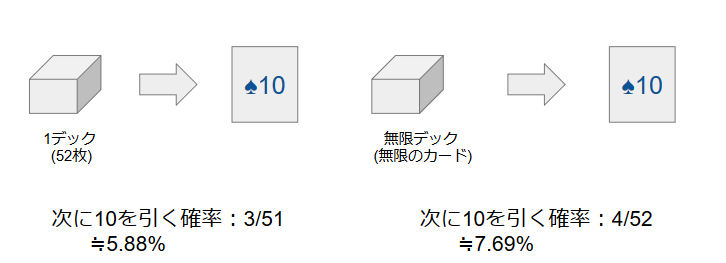
\includegraphics[width=0.7\linewidth]{./figure/DeckDiff.PNG}
 \caption{デック数による勝率の違い \label{hogehoge}}
\end{center}
\end{figure}

\bunseki{※尾崎拓海}

\section{仮説}
今回は仮説を以下のように設定した。
\begin{itemize}
\item 勝率に関して
    \begin{itemize}
        \item 仮説1.デック数が無限の時にはベーシックストラテジーの方が勝率が高い
        \item 仮説2.デック数が1の時にはベーシックストラテジー以外の勝率が高い
    \end{itemize}
\item 複雑性を考慮した場合
    \begin{itemize}
        \item 仮説3.プレイヤーの合計値が15,16,17,18以上になるまでヒットする戦略の方が性能が高い
    \end{itemize}
\item デック数を考慮した場合
    \begin{itemize}
        \item 仮説4.デック数1とデック数無限では勝率に有意な差が出る
    \end{itemize}
\end{itemize}
ベーシックストラテジーの表はデック数が無限であることを前提として導出されている。我々はこの点に着目し、デック数が有限になった際にはベーシックストラテジーよりも優れた戦略が存在するのではないか、あるいは、ベーシックストラテジーはデック数有限には対応しきれないのではないかと考えた。こうした考えから仮説1、仮説2のそれぞれを設定した。また、基準値以上になるまでヒットする戦略の方が複雑性が低くなり、性能の評価がよくなるのではないかという考えから仮説3を設定した。デック数1とデック数無限では,カードを引く確率が変化する事から、デック数が違えば勝率に有意な差が出るのではないかと考え、仮説4を設定した。
\bunseki{※尾崎拓海}

\section{検証手順}
設定した仮説を以下の手順で検証した。
\begin{enumerate}
\item ブラックジャックのシミュレータを作成
\item デック数が1の場合と無限の場合でシミュレーションを10万回実施
\item 勝った割合、負けた割合、引き分けた割合の3つを調べた
\item 得られた結果から基本戦略とその他の戦略との間の勝率に有意な差があるかどうかをカイ二乗検定を用いて調べた
\end{enumerate}
\bunseki{※尾崎拓海}

\section{ブラックジャックシミュレータ}
ベーシックストラテジーとその他の戦略を比較する事を目的に、ブラックジャックのシミュレータをプログラミング言語(Python3)を用いて作成した。このシミュレータを使用して、ベーシックストラテジー、ベーシックストラテジー改変1、ベーシックストラテジー改変2、15以上になるまでヒットする戦略、16以上になるまでヒットする戦略、17以上になるまでヒットする戦略、18以上になるまでヒットする戦略のそれぞれについて勝利回数、敗北回数、引き分けた回数の3つを調べた。ここでは、シミュレータ内部の詳細を記述していく。

\lstset{ 
   basicstyle={\ttfamily\small}, %書体の指定 
   frame=tRBl, %フレームの指定 
   framesep=10pt, %フレームと中身(コード)の間隔 
   breaklines=true, %行が長くなった場合の改行 
   linewidth=12cm, %フレームの横幅 
   lineskip=-0.5ex, %行間の調整 
   tabsize=2 %Tabを何文字幅にするかの指定 
}

\bunseki{※尾崎拓海}

\subsubsection{基本設計}
まず初めに、シミュレータの基本設計について説明する。今回作成したシミュレータではブラックジャックを行う際に必要となる要素をクラスとして表現した。具体的にはトランプのカードを
表現するカードクラスとそれを一纏めにするデッククラス、ゲーム参加者を表すクラスとそれを継承したプレイヤークラスとディーラークラス、ゲームの勝敗を判定するマネージャークラスのそれ
ぞれを定義した。これらのクラスを用いてブラックジャックのゲームを再現し、ベーシックストラテジーとその他の戦略を実行するプログラムを作成した。次に各クラスの詳細を記述していく。

\subsubsection{トランプのカードを表現するクラス}
このクラスでは実際のトランプのカードを表現するためにrankという変数にA~Kというトランプのランクを、suitという
変数にスペード、ハート、ダイヤ、クラブのスートを定義した。また、J,Q,K,Aの絵札カードは10や11と数える必要があっ
たので、ランクを数字に変換する処理もこのクラスに書き、valueという変数に入力した。ソースコードは以下である。
\begin{itemize}
\item カードを表現するクラス
\begin{lstlisting}
class Card:
    RANKS = ('A', '2', '3', '4', '5', '6', '7', '8', '9', '10', 'J', 'Q', 'K')
    SUITS = ('Spade', 'Heart', 'Diamond', 'Club')

    # 初期化
    def __init__(self, rank, suit):
        self.rank = rank
        self.suit = suit
        self.value = int(self.getvalue())

    # ランクを数字に変換する
    def getvalue(self):
        if self.rank == 'A':
            return 11
        elif self.rank == 'J' or self.rank == 'Q' or self.rank == 'K':
            return 10
        else:
            return self.rank
\end{lstlisting}
\end{itemize}

\subsubsection{デックを表現するクラス}
このクラスでは先程定義したカードクラスを利用してデックを定義した。具体的には先程のカードクラスの配列を作成
し、その中にジョーカーを除く52種類のトランプカードを作成した。このクラスの初期化時に使用するデックの数を指
定する。また、デックのシャッフルには独自に作成した関数を使用した。このシャッフル関数はPython3のrandom関数を
用いて独自に設計したものであり、引数にシャッフルを行う回数を指定する。カードの配列の長さが仮に52だった場合に
は、1~26番目のカードからランダムに取り出したカードと、27~52番目のからランダムに取り出したカードを交換する
という処理を(デック数×指定されたシャッフル回数)繰り返すという処理でシャッフル関数を作成した。ソースコードは以下である。
\begin{itemize}
\item デックを表現するクラス
\begin{lstlisting}
class Deck:
    CARDS = [Card(rank, suit) for suit in Card.SUITS for rank in Card.RANKS]
    Cards = []
    BaseDeck = []
    for rank in Card.RANKS:
        for suit in Card.SUITS:
            # オブジェクト共有を回避するための基本となる一デッキ
            BaseDeck.append(Card(rank, suit))  

    # 初期化
    # decNum の数だけデッキを使用する
    def __init__(self, decNum):
        basedec = []
        while (decNum > 0):
            basedec += self.BaseDeck
            decNum -= 1
        self.Cards = basedec
        self.current = 0

    # シャッフルをする関数
    # 引数に入れる数字によりシャッフルの回数を制御
    def shuffle(self, shuffleNum):
        self.current = 0
        while shuffleNum > 0:
            cut1 = random.randrange(0, len(self.Cards) / 2)
            cut2 = random.randrange(len(self.Cards) / 2, len(self.Cards))
            temp = self.Cards[cut1]
            self.Cards[cut1] = self.Cards[cut2]
            self.Cards[cut2] = temp
            shuffleNum -= 1
\end{lstlisting}
\end{itemize}

\subsubsection{ゲーム参加者を表すスーパークラス}
このクラスでは自身の手札とその手札の合計値、手札に含まれるAの枚数、バーストしているかどうかのフラグ、手札
がブラックジャックとなっているかどうかのフラグのそれぞれを定義している。手札に含まれるAの枚数は自身の手札
の合計値を計算する時と、ブラックジャックの条件を満たしているかどうかを判別する際に使用した。また手札の合計
値を返す関数を定義し、その内側で自身がバーストしているかどうかの判定も行っている。ソースコードは以下である。
\begin{itemize}
\item ゲーム参加者を表すスーパークラス
\begin{lstlisting}
class GamePlayer:

    # 初期化関数
    def __init__(self):
        # 参加者の手札
        self.cards = []  
        # 参加者の手札の合計値
        self.total = 0  
        # 参加者の手札に含まれるAの枚数
        self.acetotal = 0  
        # 1として数えたAの枚数
        self.usedace = 0  
        # バーストしているかどうか
        self.burst = False  
        # ナチュラルブラックジャックを満たしているかどうか
        self.naturalbj = False 
        # 手札の合計値が21 になっているかどうか
        self.normalbj = False  

    # 子オブジェクトから呼び出せる初期化関数
    def initialize(self):
        self.cards = []
        self.total = 0
        self.acetotal = 0
        self.usedace = 0
        self.burst = False
        self.naturalbj = False
        self.normalbj = False

    # ゲームプレイヤーの手札の合計値を返す関数
    def totalvalue(self):
        i = 0
        self.total = 0
        self.acetotal = 0
        cardnum = len(self.cards)

        while i < cardnum:
            if (self.cards[i].rank == 'A'):
                self.acetotal += 1
            self.total += self.cards[i].value
            i += 1
        self.total -= 10 * self.usedace

        # プレイヤーのバースト判定の処理
        if (self.total > 21):
            if (self.acetotal - self.usedace > 0):
                self.total -= 10
                self.usedace += 1
                if (self.total > 21):
                    self.burst = True
            else:
                self.burst = True

\end{lstlisting}
\end{itemize}

\subsubsection{プレイヤークラス}
このクラスは先のゲーム参加者を表すスーパークラスを継承しており、ゲームに参加しているプレイヤーを表現して
いる。プレイヤークラスでは新たに自身の名前を表す変数と自身の勝利回数、敗北回数を記録する変数を定義した。
またこのクラスでは新しく、カードを受け取る関数とヒットを行う関数、スタンドを行う関数、勝利回数と敗北回数
を増加させる関数を作成した。ソースコードは以下である。
\begin{itemize}
\item プレイヤークラス
\begin{lstlisting}
class Player(GamePlayer):
    # プレイヤーの初期化
    def __init__(self, name):
        self.name = name  # プレイヤーの名前
        self.totalwin = 0  # プレイヤーの勝利回数
        self.totallose = 0  # プレイヤーの敗北回数
        super().__init__()

    # プレイヤーがカードを受け取る時に使用する関数
    def dealedcard(self, card):
        self.cards.append(card)

    # プレイヤー側のヒットの処理
    def hit(self, dealer):
        self.dealedcard(dealer.dealcard())
        self.showhands()

    # プレイヤー側のスタンドの処理
    def stand(self):
        pass

    # プレイヤーの勝利回数を増やす
    def addtotalwin(self):
        self.totalwin += 1

    # プレイヤーの敗北回数を増やす
    def addtotallose(self):
        self.totallose += 1

\end{lstlisting}
\end{itemize}

\subsubsection{ディーラークラス}
このクラスは先のゲーム参加者を表すスーパークラスを継承しており、ゲームのディーラーを表現しているクラス
となっている。ディーラークラスの中でデックをインスタンス化してディーラー側がデックを所持している事を表
現している。このクラスでは新しく、デックのシャッフル回数という変数を定義した。また、このクラスではカード
を配る関数、ディーラーの手札合計が17を超えるまでカードを引き続ける関数を作成した。カードを配る関数についてはデック数有限の時とデック数無限の時とで処理を変更している。ソースコードは以下である。
\begin{itemize}
\item ディーラークラス(デック数有限)
\begin{lstlisting}
class Dealer(GamePlayer):
    # ディーラーの初期化
    def __init__(self, deckNum):
        self.deck = Deck(deckNum)
        # ディーラーがシャッフルする回数。今回は一万回シャッフルする。
        self.shufflenum = 10000
        self.deck.shuffle(deckNum * self.shufflenum)
        super().__init__()

    # カードを配る関数
    def dealcard(self):
        ''' デック数有限の際はこちらのコメントアウトを解除する '''
        card = self.deck.Cards[self.deck.current]
        self.deck.current += 1
        
        ''' デック数無限の際にはこちらのコメントアウトを解除する '''
        # randomcard = random.randrange(13);
        # card = Card(Card.RANKS[randomcard], Card.SUITS[0])
        # return card

    # 一番最初にカードを配る際の関数
    def firstdeal(self, player):
        super().__init__()
        for x in player:
            x.initialize()
        firstdeal = 2
        while firstdeal > 0:
            self.cards.append(self.dealcard())
            for x in player:
                x.cards.append(self.dealcard())
            firstdeal -= 1

    # 合計が17 を超えるまで引き続ける処理
    def continuehit(self):
        self.totalvalue()
        while (self.total < 17):
            self.cards.append(self.dealcard())
            self.totalvalue()

\end{lstlisting}
\end{itemize}

\subsubsection{ゲームマネージャークラス}
このクラスは主にゲームの勝敗判定に使用している。プレイヤーとディーラーの手札の合計値を比較し勝敗を判定
する関数と、手札がブラックジャックになっているかどうかを判定する関数を作成した。勝敗判定のタイミングで
プレイヤーの勝利回数、敗北回数のそれぞれを記録している。ソースコードは以下である。
\begin{itemize}
\item ゲームマネージャークラス
\begin{lstlisting}
class GameManager:
    def __init__(self, players, dealer):
        self.players = players
        self.dealer = dealer
        self.checkdeal = True

    # 各プレイヤーとディーラーとの間で勝敗を決める
    def judge(self):
        for x in self.players:
            self.checkblackjack(x)
        self.checkblackjack(self.dealer)
        for player in self.players:
            if player.burst == True:
                player.addtotallose()
            elif player.burst == False and self.dealer.burst == True:
                player.addtotalwin()
            elif player.total > self.dealer.total:
                player.addtotalwin()
            elif player.total < self.dealer.total:
                player.addtotallose()
            elif player.total == self.dealer.total:
                if player.naturalbj and self.dealer.naturalbj:
                elif player.naturalbj and self.dealer.normalbj:
                    player.addtotalwin()
                elif player.normalbj and self.dealer.naturalbj:
                    player.addtotallose()
                elif player.normalbj and self.dealer.normalbj:
                    pass
                else:
                    pass
\end{lstlisting}
\end{itemize}

\subsubsection{メイン関数}
以上のクラスを用いてメイン関数にブラックジャックのゲームを記述した。以下にプログラムの実行手順を示す。
\begin{enumerate}
    \item ゲームに参加するプレイヤーを作成。今回はプレイヤーを一人のみ作成した。
    \item ディーラーを作成。
    \item カットカードを定義。カットカードを挟む位置はデックの半分の位置とした。
    \item ゲーム全体の実行回数を定義。今回は10万回とした。
    \item プレイヤーの戦略を配列形式で定義した。
    \item ゲームを繰り返すwhile文を作成し、ループ回数を10万回とした。
    \begin{enumerate}
        \item デックからカットカードが出てきたかを確認する。もし出てきていればデックをシャッフルする。
	  \item ディーラーが自身を含む各プレイヤーに初期カードを配る。
	  \item プレイヤーは自身の戦略に沿った行動を選択する。
	  \item すべてのプレイヤーの行動が終了したことを確認後にディーラーが行動を開始する
	  \item ディーラーの行動終了後に、勝敗判定を行う。
    \end{enumerate}
\end{enumerate}

\subsubsection{未実装の機能について}
今回のシミュレーションでは条件を簡単にするためにヒットとスタンドの処理のみを使用しており、ダブルダウン、スプリット、サレンダー、インシュランス、イーブンマネーについては実装していない。ブラックジャックのすべてのルールをプログラム上に再現できているわけではな
いので、後期の活動でダブルダウン、スプリット、サレンダー、インシュランス、イーブンマネーを追加した完全版のシミュレータを作成する。
\bunseki{※尾崎拓海}

\section{シミュレータの擬似乱数の検証}
今回シミュレータを作成するにあたり、擬似乱数を使用した。この擬似乱数が適切かどうかについて検証する。今回使用した擬似乱数生成方法はPython3のrandom関数である。Python Software Foundation(2018)によればrandomの擬似乱数を生成するアルゴリズムはメルセンヌツイスタを用いている。今回は周期と広井誠(2007)の等確率性の検定を行う。
\bunseki{※柿崎大輝}
\subsection{周期}
擬似乱数には周期が存在する。周期とは同じ数列が出てくるようになるまでの数字の出現回数のことを指す。周期が小さいとよく同じ数列が出てきてしまいランダム性が低い。つまり周期が大きいとランダム性が高いので、性能が良いということになる。松本眞(2013)ではメルセンヌツイスタの周期は$2^{19937}-1$である。これはほかの擬似乱数に比べ、かなり大きい周期である。そのため、メルセンヌツイスタを擬似乱数として使うのに十分であると考えられる。
\bunseki{※柿崎大輝}
\subsection{等確率性の検定}
等確率性とはどの値も等しい確率で出てくるかどうかである。カイ2乗検定を使い等確率性を検証する。random関数を使用して、0~1の範囲
の乱数を生成する。その後、その値を0~0.1、0.1~0.2、0.2~0.3、0.3~0.4、0.4~0.5、0.5~0.6、0.6~0.7、0.7~0.8、0.8~0.9、0.9~1.0の10通りに分類する。それをまとめると表\ref{table:randomresult}になる。
\begin{table}[H]
 \caption{random関数での結果}
 \label{table:randomresult}
 \begin{center}
  \begin{tabular}{|c|c|c|c|c|c|c|c|c|c|}
    \hline    0~0.1 &  0.1~0.2 & 0.2~0.3 & 0.3~0.4 &  0.4~0.5 & 0.5~0.6 & 0.6~0.7 & 0.7~0.8 & 0.8~0.9 & 0.9~1.0 \\
    \hline 95 & 85 & 100 & 102 & 91 & 114 & 87 & 108 & 115 & 103 \\
    \hline
  \end{tabular}
 \end{center}
\end{table}
完璧なランダムなのであれば、この結果はどれも100になることが予想できる。しかし、実際はすべてが100にはならないので、カイ2乗検定を行い検証する。先ほど出た度数を実現度数として使用し、100を理論度数としてカイ2乗検定を行う。この時、自由度は9で有意水準を5%とすると、棄却値は16.92となり、カイ2乗値がこれより小さいと擬似乱数が等しく出てきたといえる。実際に計算すると、カイ2乗値は9.98となった。この値は16.92より小さいので、擬似乱数によって出た値はすべて等しい確率で出てきたといえる。

以上のことから、メルセンヌツイスタは周期が大きいこととカイ2乗検定で値が全て等しい確率で出ていることから十分に使えると判断することができるため、今回のシミュレータにおいて使用した。
\bunseki{※柿崎大輝}
\chapter{検証結果}
\section{シミュレーション結果まとめ}
シミュレータで10万回ブラックジャックを行った結果を表1に示す。
\begin{table}[H]
 \caption{デック数と各戦略での勝利、負け、引き分け}
 \begin{center}
  \begin{tabular}{|c|c|c|c|c|c|c|}
    \hline & \multicolumn{3}{c|}{デック数無限} & \multicolumn{3}{c|}{デック数1} \\
    \cline{2-7} & 勝ち & 負け & 引き分け & 勝ち & 負け & 引き分け \\
    \hline ベーシックストラテジー & 42746 & 48635 & 8619 & 43111 & 48654 & 8235 \\
    \hline ベーシックストラテジー改変1 & 42583 & 48782 & 8635 & 42923 & 48909 & 8168 \\
    \hline ベーシックストラテジー改変2 & 42223 & 49079 & 8698 & 42955 & 48689 & 8356 \\
    \hline 15以上 & 42392 & 49458 & 8150 & 42063 & 50027 & 7910 \\
    \hline 16以上 & 41410 & 49506 & 9084 & 41580 & 49672 & 8748 \\
    \hline 17以上 & 40870 & 49400 & 9730 & 40974 & 49630 & 9396 \\
    \hline 18以上 & 39291 & 52587 & 8122 & 42071 & 49872 & 8057 \\
    \hline
  \end{tabular}
 \end{center}
\end{table}
今回シミュレータで各戦略を10万回実行してみた。その結果を勝ち、負け、引き分けの3種類に分けて、表にまとめた。縦軸はデックの数とそれに対応する勝敗とし、横軸は戦略ごとに分けている。例えば、ベーシックストラテジーでデック数1の場合を見ると勝ちが43111で負けが48654で引き分けが8235となっている。またデック数1の勝ちを全体でみると最も多いことが分かる。\\
全体として勝ちの数は4万回前後に収まっており、負けの数は5万回前後に収まっている。基本的に負けの数のほうが多いことが分かる。デック数で比べると、ほとんどの戦略でデック数1の場合のほうが勝ちの数が多いということが発見される。また、デック数に関係なく、勝ちの数はベーシックストラテジーが一番多いということが分かる。
\bunseki{※柿崎大輝}
\section{検定}
先ほどのシミュレータの結果からベーシックストラテジーが最も勝率が高いというを確かめるために、戦略の間の勝率に有意な差があるかどうかを確かめたい。また、デック数によって勝率が変化するということも確かめるために、デック数の違いによって戦略の勝率に有意な差があるかも確かめたい。確かめるために検定を行う。
\bunseki{※柿崎大輝}
\subsection{カイ2乗検定の独立性の検定}
勝率に有意な差があるかどうかを確かめるためカイ2乗検定の独立性の検定を使用する。カイ2乗検定ではカイ2乗値を用いて検定を行う。カイ2乗値は下の式で計算を行う。
\begin{equation} カイ2乗 = \sum{ \frac{(実現度数 - 理論度数)^2}{理論度数}} \end{equation}
実現度数とは実際に出た度数のことで、理論度数は理想としてでる度数のことである。実現度数はシミュレータの結果から参照し、理論度数はシミュレータの結果から計算する。
理論度数は以下の式で計算される。
\begin{equation} 理論度数 =  行の合計 \frac{列の合計}{すべての合計} \end{equation}
\bunseki{※柿崎大輝}
\subsubsection{戦略間の勝率}
カイ2乗検定を行うためにシミュレータの結果の表を変形する。
\begin{table}[H]
 \caption{デック数無限の場合}
 \begin{center}
  \begin{tabular}{|c|c|c|c|}
    \hline
      & 勝ち & 勝ち以外(負けと引き分け) & 合計 \\
    \hline ベーシックストラテジー (実現度数)& 42746 & 57254 & 100000 \\
             ベーシックストラテジー (理論度数)& 41645 & 58355 &  \\
    \hline ベーシックストラテジー改変1 (実現度数)& 42583 & 57417 & 100000 \\
             ベーシックストラテジー改変1 (理論度数)& 41645 & 58355 &  \\
    \hline ベーシックストラテジー改変2 (実現度数)& 42223 & 57777 & 100000 \\
              ベーシックストラテジー改変2 (理論度数)& 41645 & 58355 &  \\
    \hline 15以上 (実現度数)& 42392 & 57608 & 100000 \\
             15以上 (理論度数)& 41645 & 58355 &  \\
    \hline 16以上 (実現度数)& 41410 & 58590 & 100000 \\
             16以上 (理論度数)& 41645 & 58355 &  \\
    \hline 17以上 (実現度数)& 40870 & 59130 & 100000 \\
             17以上 (理論度数)& 41645 & 58355 &  \\
    \hline 18以上 (実現度数)& 39291 & 60709 & 100000 \\
             18以上 (理論度数)& 41645 & 58355 &  \\
    \hline  合計 & 291515 & 408485 & 700000 \\
    \hline
  \end{tabular}
 \end{center}
\end{table}
\begin{table}[H]
 \caption{デック数1の場合}
 \begin{center}
  \begin{tabular}{|c|c|c|c|}
    \hline
      & 勝ち & 勝ち以外(負けと引き分け) & 合計 \\
    \hline ベーシックストラテジー (実現度数)& 43111 & 56889 & 100000 \\
             ベーシックストラテジー (理論度数)& 42240 & 57760 &  \\
    \hline ベーシックストラテジー改変1 (実現度数)& 42923 & 57077 & 100000 \\
             ベーシックストラテジー改変1 (理論度数)& 42240 & 57760 &  \\
    \hline ベーシックストラテジー改変2 (実現度数)& 42955 & 57045 & 100000 \\
              ベーシックストラテジー改変2 (理論度数)& 42240 & 57760 &  \\
    \hline 15以上 (実現度数)& 42063 & 57937 & 100000 \\
             15以上 (理論度数)& 42240 & 57760 &  \\
    \hline 16以上 (実現度数)& 41580 & 58420 & 100000 \\
             16以上 (理論度数)& 42240 & 57760 &  \\
    \hline 17以上 (実現度数)& 40974 & 59026 & 100000 \\
             17以上 (理論度数)& 42240 & 57760 &  \\
    \hline 18以上 (実現度数)& 42071 & 57045 & 100000 \\
             18以上 (理論度数)& 42240 & 57760 &  \\
    \hline  合計 & 295677 & 404323 & 700000 \\
    \hline
  \end{tabular}
 \end{center}
\end{table}
シミュレーション結果の表を改変したもので、負けと引き分けをまとめ、縦軸と横軸の合計を使用して、理論度数を計算して付け加えたものである。
カイ2乗検定を行う前に帰無仮説、対立仮説と有意水準を定める。\\
帰無仮説:戦略間の勝率に有意な差がない\\
対立仮説:戦略間の勝率に有意な差がある\\
有意水準を5%として、カイ2乗検定を行う。\\
自由度は(行の数-1)(列の数-1)で求められるので、(7-1)(2-1)で自由度6となる。自由度6かつ有意水準5%の時、棄却値は12.96となる。この棄却値よりもカイ2乗値が大きい場合、帰無仮説を棄却して対立仮説が採択される。\\
デック数無限の場合、カイ2乗値は377.8012となり、カイ2乗値が12.96より大きい377.8012となるため、帰無仮説を棄却する。つまり、デック数無限の場合、勝率に有意な差が存在する。\\
デック数1の場合、カイ2乗値は127.8811となり、カイ2乗値が12.96より大きい127.8811となるため帰無仮説を棄却する。つまり、デック数1の場合、勝率に有意な差が存在する。
\bunseki{※柿崎大輝}
\subsubsection{デック数による勝率}
カイ2乗検定を行うための表を作成する。まずがベーシックストラテジーでの表を作成する。
\begin{table}[H]
 \caption{デック数ごとのベーシックストラテジー}
 \begin{center}
  \begin{tabular}{|c|c|c|c|}
    \hline
      & 勝ち & 勝ち以外(負けと引き分け) & 合計 \\
    \hline デック数無限のベーシックストラテジー (実現度数)& 42798 & 57202 & 100000 \\
            デック数無限のベーシックストラテジー (理論度数)& 42955 & 57046 &  \\
    \hline デック数1のベーシックストラテジー (実現度数)& 43111 & 56889 & 100000 \\
            デック数1のベーシックストラテジー (理論度数)& 42955 & 57046 &  \\
    \hline  合計 & 85909 & 114991 & 200000 \\
    \hline
  \end{tabular}
 \end{center}
\end{table}
7つの戦略のうち1つ対象にして、デック数無限とデック数1の場合の勝ちと勝ち以外の2つを載せ、それに合計と理論度数を付け足した表である。縦軸は勝敗で横軸はデック数での戦略である。
シミュレータの結果からこのような表を7つの戦略で作る。
カイ2乗検定を行う前に帰無仮説、対立仮説と優位水準を定める。\\
帰無仮説:デック数1とデック数無限の勝率に有意な差がない\\
対立仮説:デック数1とデック数無限の勝率に有意な差がある\\
優位水準を5%として、カイ2乗検定を行う。\\
自由度は1となり、優位水準5%なので、棄却値は3.84となる。この棄却値よりもカイ2乗値が大きい場合、帰無仮説を棄却して対立仮説が採択される。\\
ベーシックストラテジーの場合、カイ2乗値は1.0665となり、カイ2乗値が3.84より小さい1.0665となるため、帰無仮説を棄却しない。つまり、ベーシックストラテジーでデック数が1と無限では勝率に有意な差はない。
これをそれぞれベーシックストラテジー改変1、ベーシックストラテジー改変2、15以上、16以上、17以上、18以上について同じように行う。
すべてをまとめると、ベーシックストラテジー改変1から順にカイ2乗値は4.6112、3.0753、2.2164、0.5952、0.2237、160.1305となった。この中で棄却値3.84を超えたのはベーシックストラテジー改変1と18以上の場合である。ベーシックストラテジー改変2、15以上、16以上と17以上の場合、デック数が1と無限では勝率に有意な差はない、ベーシックストラテジー改変1と18以上の場合、デック数が1と無限では勝率に有意な差はあるという結果である。
\bunseki{※柿崎大輝}
\subsection{残差分析}
カイ2乗検定によって各戦略間の勝率に有意な差が存在することが判明した。しかし、どこに有意な差が存在するのかが分からない。そのためさらに検定を行いどの戦略
に有意な差が存在するのかを探す。有意な差がどこに存在するのかを発見するため残差分析を行う。残差分析では調整済み標準化残差を算出し、調整済み標準化残差が1.96
より大きい場合と-1.96より小さい場合に有意な差があると分かる。調整済み標準化残差は以下の式で計算される。
\begin{equation} 調整済み標準化残差 =  \frac{\frac{実現度数 - 理論度数}{\sqrt{理論度数}}}{(1-行比率)(1-列比率)} \end{equation}
調整済み標準化残差をそれぞれ出したものを表でまとめる。
\begin{table}[H]
 \caption{調整済み標準化残差}
 \begin{center}
  \begin{tabular}{|c|c|c|c|c|}
    \hline
     & \multicolumn{2}{c|}{デック数無限} & \multicolumn{2}{c|}{デック数1} \\
    \cline{2-5} & 勝ち & 勝ち以外 & 勝ち & 勝ち以外 \\
    \hline ベーシックストラテジー & 7.63 & -7.63 & 6.02 & -6.02  \\
    \hline ベーシックストラテジー改変1 & 6.50 & -6.50 & 4.73 & -4.73  \\
    \hline ベーシックストラテジー改変2 & 4.00 & -4.00 & 4.95 & -4.95  \\
    \hline 15以上 & 5.18 & -5.18 & -1.22 & 1.22  \\
    \hline 16以上 & -1.63 & 1.63 & -4.56 & 4.56  \\
    \hline 17以上 & -5.37 & 5.37 & -8.75 & 8.75  \\
    \hline 18以上 & -16.31 & 16.31 & -1.17 & 1.17  \\
    \hline
  \end{tabular}
 \end{center}
\end{table}
この表ではそれぞれの戦略でのデック数無限と1の場合の勝ちと勝ち以外の調整済み標準化残差を示している。縦軸がデック数とデック数に対応した勝ちと勝ち以外の項目で、横軸がそれぞれの戦略に分かれている。この表の1.92以上と-1.92以下が有意な差とある判断できる。例えば、デック数無限の勝ちでベーシックストラテジーをみると値が7.63になっており、1.92以上なのでベーシックストラテジーの勝ちの数はほかの戦略の勝ちより有意に多かったということが分かる。\\
デック数無限を見ると、ベーシックストラテジーやベーシックストラテジー改変1、ベーシックストラテジー改変2、15以上になるまでヒットする戦略での勝ちの項目が1.96を超えておりほかの戦略より有意に多いことが分かる。逆に17以上までヒットする戦略と18以上までヒットする戦略は勝ちの項目が-1.96を下回ったのでほかの戦略より有意に少ない。
デック数1を見ると、ベーシックストラテジーやベーシックストラテジー改変1、ベーシックストラテジー改変2の勝ちの項目が1.96を超えておりほかの戦略より有意に多いことが分かる。逆に16以上までヒットする戦略と17以上までヒットする戦略は勝ちの項目が-1.96を下回ったのでほかの戦略より有意に少ない。
ベーシックストラテジー、ベーシックストラテジー改変1、ベーシックストラテジー改変2の3つはデック数に関係なく勝ちが有意に多いことが分かる。逆に、17以上までヒットする戦略はデック数にかかわりなく勝ちが有意に少ないことが分かる。
\bunseki{※柿崎大輝}
\subsection{多重比較}
残差分析によって全戦略のどこに有意な差があるかが分かった。しかし、戦略と戦略の間に有意な差があるかはわからない。そのため、多重比較を行い、戦略間に有意な差があるかどうかを確認する。\\
fisherの正確確率検定を用いて、戦略間のp値をすべて算出し、p値をholm法で調整を施す。p値が0.05以下の場合、有意な差がある。p値が0.05より大きい場合、有意な差がないとする。それを表にまとめた。
\begin{table}[H]
 \caption{デック数無限の多重比較}
 \begin{center}
 \small
 \scalebox{0.7}[1.0]{
  \begin{tabular}{|c|c|c|c|c|c|c|}
    \hline & ベーシックストラテジー & ベーシックストラテジー改変1 & ベーシックストラテジー改変2 & 15以上 & 16以上 & 17以上 \\
    \hline ベーシックストラテジー改変1 勝率差 & 0.1 &  &  &  &  &   \\
    ベーシックストラテジー改変1 p値 & 1.000 &  &  &  &  &    \\
    \hline ベーシックストラテジー改変2 勝率差 & 0.5 & 0.4 & & & &  \\
    ベーシックストラテジー改変2 p値 & 0.109 & 0.522 & & & &   \\
    \hline 15以上 勝率差 & 0.3 & 0.2 & -0.2 & & &   \\
    15以上 p値 & 0.522 & 1.000 & 1.000 & & &  \\
    \hline 16以上 勝率差 & 1.3 & 1.2 & 0.8 & 1.0 & &  \\
    16以上 p値 & 0 & 0 & 0.002 & 0 & &  \\
    \hline 17以上 勝率差 & 1.8 & 1.8 & 1.3 & 1.5 & 0.5 &  \\
    17以上 p値 & 0 & 0 & 0 & 0 & 0 & \\
    \hline 18以上 勝率差 & 3.4 & 3.3 & 2.9 & 3.1 & 2.1 & 1.6  \\
    18以上 p値 & 0 & 0 & 0 & 0 & 0 & 0  \\
    \hline
  \end{tabular}
 }
 \end{center}
\end{table}
\begin{table}[H]
 \caption{デック数1の多重比較}
 \begin{center}
 \small
 \scalebox{0.7}[1.0]{
  \begin{tabular}{|c|c|c|c|c|c|c|}
    \hline & ベーシックストラテジー & ベーシックストラテジー改変1 & ベーシックストラテジー改変2 & 15以上 & 16以上 & 17以上 \\
    \hline ベーシックストラテジー改変1 勝率差 & 0.2 &  &  &  &  &   \\
    ベーシックストラテジー改変1 p値 & 1.000 &  &  &  &  &    \\
    \hline ベーシックストラテジー改変2 勝率差 & 0.1 & -0.1 & & & &  \\
    ベーシックストラテジー改変2 p値 & 1.000 & 1.000 & & & &   \\
    \hline 15以上 勝率差 & 1.0 & 0.8 & 0.9 & & &   \\
    15以上 p値 & 0 & 1.001 & 0.001 & & &  \\
    \hline 16以上 勝率差 & 1.5 & 1.3 & 1.4 & 0.5 & &  \\
    16以上 p値 & 0 & 0 & 0 & 0.158 & &  \\
    \hline 17以上 勝率差 & 2.1 & 2.1 & 2.0 & 1.1 & 0.6 &  \\
    17以上 p値 & 0 & 0 & 0 & 0 & 0.042 & \\
    \hline 18以上 勝率差 & 1.0 & 1.0 & 0.9 & 0 & -0.5 & -1.1 \\
    18以上 p値 & 0 & 0.001 & 0.001 & 1.000 & 0.158 & 0  \\
    \hline
  \end{tabular}
 }
 \end{center}
\end{table}
表にはそれぞれの戦略を比較した場合の勝率差とp値の2つの項目で構成されており、勝率差がプラスの場合、縦軸の戦略のほう勝率が良いことになる。例えば、縦軸がベーシックストラテジー、横軸が15以上になるまでヒットする戦略の部分を見ると、勝率が1.0でp値が0となっている。p値が0.05より小さいためベーシックストラテジーと15以上になるまでヒットする戦略の間の勝率に有意な差が存在することになり、ベーシックストラテジーのほうが勝率が1.0高いということになる。
表により、デック数無限の場合、ベーシックストラテジー、ベーシックストラテジー改変1、ベーシックストラテジー改変2と15以上になるまでヒットする戦略の4つで勝率に有意な差がない。16以上までヒットする戦略と17以上までヒットする戦略の2つは勝率に有意な差はない。それ以外には勝率に有意な差が存在した。これらを勝率の高い順に戦略を並べると、ベーシックストラテジーなどの戦略、16と17以上までヒットする戦略、18以上までヒットする戦略となる。デック数1の場合はベーシックストラテジー、ベーシックストラテジー改変1とベーシックストラテジー改変2の3つに勝率に有意な差が存在しない。15以上になるまでヒットする戦略、16以上になるまでヒットする戦略と18以上になるまでヒットする戦略の3つに有意な差が存在しない。これらを勝率の高い順に戦略を並べると、ベーシックストラテジーとベーシックストラテジー改変1ベーシックストラテジー改変2の戦略、15と16と18以上になるまでヒットする戦略、17以上までヒットする戦略となる。
\bunseki{※柿崎大輝}

\section{複雑性を考慮した性能比較とその結果}

本項では、複雑性を考慮した性能比較について、また、その結果について説明する。

\subsection{複雑性の定義について}

より人に扱いやすい戦略を定義する為に、A.N. Kolmogorov氏の『On tables of random numbers』を参考にし、戦略の複雑性を次のように設定した。
まず、戦略の文字列を圧縮する。圧縮の方法は、「連続する文字+連続して文字が出た回数」を合わせたものとした。例として、「HHSSSHHHHH」という10字からなる文字列を圧縮すると、「H2S3H5」となり、圧縮した後の文字列は6字となる。この時、連続して文字が出た回数が2桁になったとしても、ここでは1字として数える。

\subsection{各戦略の複雑性}

この圧縮の方式を各戦略に行い、それぞれの圧縮された後の文字列の長さを元の長さで割ったものを複雑性とした。用意した戦略は次のような8行の配列とし、それぞれの行に圧縮を行った。\\

%\begin{figure}[htbp]
%\begin{center}
%\includegraphics[width=15cm,bb=0 0 602 281]{1.png}
%\end{center}
%\caption{基本戦略の戦略表}
%\label{picture}
%\end{figure}

\begin{table}[H]
\caption{基本戦略の戦略表}
\label{table:data_type}
\begin{center}
\begin{tabular}{llllllllllll}
\hline
			     &              & \multicolumn{10}{c}{ディーラーのアップカード}      \\ \cline{3-12} 
                        &              & 2 & 3 & 4 & 5 & 6 & 7 & 8 & 9 & 10 & A \\ \hline
{手札の合計}  & 19以上        & S & S & S & S & S & S & S & S & S  & S \\
                        & 18          & S & S & S & S & S & S & S & S & S  & S \\
                        & 17          & S & S & S & S & S & S & S & S & S  & S \\
                        & 16          & S & S & S & S & S & H & H & H & H  & H \\
                        & 15          & S & S & S & S & S & H & H & H & H  & H \\
                        & 13$\sim$14  & S & S & S & S & S & H & H & H & H  & H \\
                        & 12          & H & H & S & S & S & H & H & H & H  & H \\
                        & 11以下        & H & H & H & H & H & H & H & H & H  & H
\end{tabular}
\end{center}
\end{table}

今回用意した戦略を、全て圧縮したのが以下の表である。


%\begin{figure}[htbp]
%\begin{center}
%\includegraphics[width=15cm,bb=0 0 602 261]{2.png}
%\end{center}
%\caption{各戦略の圧縮した後の文字列と複雑性}
%\label{picture}
%\end{figure}

\begin{table}[H]
\caption{各戦略の圧縮した後の文字列と複雑性}
\label{table:data_type}
\begin{center}
\begin{tabular}{llll}
戦略           & 圧縮した後の文字列                                                                   & 文字列長 & 複雑性   \\ \hline
基本戦略         & \begin{tabular}[c]{@{}l@{}}S10S5H5S5H5S5H5S5H5S5H5H2S3H5H10\end{tabular} & 30   & 0.375 \\
基本戦略改変1      & S10S5H5S5H5S5H5S5H5S5H5S5H5H10                                              & 28   & 0.35  \\
基本戦略改変2      & S10S5H5S5H5S5H5S5H5S5H5H10H10                                               & 26   & 0.325 \\
15以上になるまでヒット & S10S10S10S10S10H10H10H10                                                    & 16   & 0.2   \\
16以上になるまでヒット & S10S10S10S10H10H10H10H10                                                    & 16   & 0.2   \\
17以上になるまでヒット & S10S10S10H10H10H10H10H10                                                    & 16   & 0.2   \\
18以上になるまでヒット & S10S10H10H10H10H10H10H10                                                    & 16   & 0.2  
\end{tabular}
\end{center}
\end{table}

この表を見ると、基本戦略を改変した戦略の方が、複雑性が低く、人にとって扱いやすいといえる。また、一定の数字以上になるまでヒットを続ける戦略は、複雑性が基本戦略の半分程度であり、とても人にとって扱いやすい戦略だといえる。

\subsection{各戦略の性能評価}

そして、今回はその複雑性を用いて、各戦略の性能比較を行った。
性能の基準は以下の二通りを用意した。\\
~~ 1. (勝率) ÷ (複雑性)\\
~~ 2. (勝率) - (複雑性)\\
この評価基準に従って、1デックの時と無限デックの時の性能を表にした。\\\\\\\\\\\\\\\\\\\\\\\\




%\begin{figure}[htbp]
%\begin{center}
%\includegraphics[width=15cm,bb=0 0 602 279]{3.png}
%\end{center}
%\caption{1デックの時の各戦略の性能}
%\label{picture}
%\end{figure}

\begin{table}[H]
\caption{1デックの時の各戦略の性能}
\label{table:data_type}
\begin{center}
\begin{tabular}{llllll}
戦略           & 圧縮長 & 勝率    & 複雑性   & 性能1  & 性能2   \\ \hline
基本戦略         & 30  & 0.431 & 0.375 & 1.14 & 0.052 \\
基本戦略改変1      & 28  & 0.429 & 0.35  & 1.22 & 0.076 \\
基本戦略改変2      & 26  & 0.430 & 0.325 & 1.21 & 0.072 \\
15以上になるまでヒット & 16  & 0.421 & 0.200 & 2.12 & 0.224 \\
16以上になるまでヒット & 16  & 0.416 & 0.200 & 2.07 & 0.214 \\
17以上になるまでヒット & 16  & 0.410 & 0.200 & 2.05 & 0.209 \\
18以上になるまでヒット & 16  & 0.421 & 0.200 & 1.97 & 0.193
\end{tabular}
\end{center}
\end{table}


%\begin{figure}[htbp]
%\begin{center}
%\includegraphics[width=15cm,bb=0 0 541 255]{4_.png}
%\end{center}
%\caption{無限デックの時の各戦略の性能}
%\label{picture}
%\end{figure}

\begin{table}[H]
\caption{1デックの時の各戦略の性能}
\label{table:data_type}
\begin{center}
\begin{tabular}{llllll}
戦略           & 圧縮長 & 勝率    & 複雑性   & 性能1  & 性能2   \\ \hline
基本戦略         & 30  & 0.427 & 0.375 & 1.14 & 0.052 \\
基本戦略改変1      & 28  & 0.424 & 0.35  & 2.12 & 0.224 \\
基本戦略改変2      & 26  & 0.414 & 0.325 & 1.07 & 0.214 \\
15以上になるまでヒット & 16  & 0.424 & 0.200 & 2.05 & 0.209 \\
16以上になるまでヒット & 16  & 0.414 & 0.200 & 1.97 & 0.193 \\
17以上になるまでヒット & 16  & 0.409 & 0.200 & 1.21 & 0.076 \\
18以上になるまでヒット & 16  & 0.393 & 0.200 & 1.21 & 0.072
\end{tabular}
\end{center}
\end{table}

各戦略を比較し、次のような結果を得た。
まず、勝率のみを考慮した場合、一定の数字以上でスタンドする戦略よりも、基本戦略とそれを改変した戦略の方が有意に高い勝率だった。
また、基本戦略と改変1、改変2のそれぞれの戦略間には有意な差が見られなかった。
複雑性を考慮して性能を評価した場合、基準値を15に設定した戦略が一番優秀であった。

\subsection{考察}

勝率のみを見ると、1デック、無限デック共に基本戦略が最も勝率が高かった。しかし、扱いやすさも含めた性能を評価すると、必ずしも基本戦略が扱いやすいとは限らず、改善の余地があるということが分かった。

\subsection{今後の課題}

前期のプロジェクト学習におけるブラックジャックの前提では、それぞれのゲームは1ゲームで行われており、過去に出たゲームが次以降のゲームに影響されることはなかった。そのため、有限のデックで連続したゲームを行った場合の戦略について考える必要がある。

また、今回は勝率のみを考えた場合を想定していた。実際のゲームでは、賭け金の概念があるので、それを導入した場合にどのように利得をプラスにするか、そのための戦略を考える必要がある。それに伴い、今回のプロジェクトでは省いたダブルダウン、スプリット、サレンダー等のルールを含めて最終的な利得をプラスにする戦略を考えたい。

戦略の扱いやすさについて、今回は複雑性の設定を手動で行い、検証する時間もあまり取らなかったので、評価基準が正確ではない可能性がある。
今後、この評価基準をどのように調整するかも検討の余地がある。

\bunseki{※渡邊凛}

\chapter{前期活動}
\section{ブラックジャックの学習}
本プロジェクトで題材としているブラックジャックというゲームを
実際のプレイも交えて学習した。前章までで説明したベーシックストラテジーを
試すということもその中で行ったが、実際に使用してみると表を覚え、かつ
素早いゲームの進行に合わせながら実行するのは容易ではないという実感が得られた.
もちろんディーラー側に戦略の実行をさとられないようにするためには、ゲームの進行を
止めるなど違和感を持たせるような行動はできるだけ無くす必要がある。以上のことから、
戦略の単純化の必要性を再確認した。
\bunseki{※米村祥裕}

\section{シミュレータの作成}
シミュレータはPython3系で作成を行った.シミュレータ作成の過程ではPython3のプログラミング
とGitによるバージョン管理について学習した。前期までで得られたブラックジャックの戦略比較に用いた
数値はこのシミュレータによって得られた。
\bunseki{※米村祥裕}

\section{統計学の学習}
シミュレータの正しさ、シミュレーション結果の分析のために統計学を学習した。
\bunseki{※米村祥裕}

\section{複雑性の学習}
本プロジェクトにおいて、戦略の複雑性を評価することはとても重要な事項である。
複雑性の定義付けのためにコルモゴロフの複雑性を参考にし、コルモゴロフ複雑性の
定義と使われ方について調査し学習した。
\bunseki{※米村祥裕}

\section{ニューラルネットワーク}
本プロジェクトでは最適な戦略の探索を行うための技術の一つとしてニューラルネットワークを
挙げ、勉強会を行った。
\bunseki{※米村祥裕}
\chapter{後期活動}
後期の目標としては次が挙げられる。

\begin{itemize}
\item ディーラー側の行動の検証
\item デックが有限個の場合での戦略
\item 賭け金の概念の導入
\item より扱いやすい戦略の検証
\end{itemize}

ディーラー側の行動の検証については、ニューラルネットワークを用いて、プレイヤーがどのような戦略を取っているのかを検知するプログラムを作成することを目標にしている。例えば、プレイヤーがカウンティング戦略を使用している際にそれを見抜く事ができるようなプログラムを作成し、そうして作成したプログラムを用いて、ディーラー側に検知されにくい戦略の生成に活用しようと考えている。

デックが有限個の場合での戦略については、実際の対戦に従って、デック数が有限でシャッフルを一定ゲーム数まで行わず、連続でゲームを行う場合の最適な戦略を検証することを目標にしている。前述したとおりベーシックストラテジーはデック数が無限であるという前提のもと成立している戦略であるが、実際のゲームにおいてはデック数は有限であり、シャッフルを一定ゲーム数まで行わない。この事から、ゲームの進行状況により、最適とされる戦略が変わる可能性がある。そのため、デック数が有限で連続してゲームを行うと設定した状態での最適な戦略について検証することを考えている。

賭け金の概念の導入では実際のブラックジャックのゲームに則って賭け金を設定し、利得をどの様にプラスにしていくか、そのための最適な行動を考える。前期の活動では賭け金の概念は考えず、戦略の勝率のみに着目していた。しかし、実際のブラックジャックのゲームにおいては戦略の勝率が低かったとしても賭け金の賭け方によっては利得をプラスにすることが可能である。この事から、戦略の勝率のみに着目するのではなく、賭け金の賭け方にも着目し、最終的な利得をプラスにしていく戦略を検証することを考えている。

より扱いやすい戦略の検証について、今回は複雑性の設定を手動で行い、検証する時間もあまり取らなかったため、評価基準が正確ではない可能性がある。今後、この評価基準をどのように調整するかも検討しようと考えている。

\bunseki{※渡邊凛}
\chapter{中間発表の評価}
\chapter{中間発表の評価}
 本章では中間発表で記入してもらった評価シートの集計結果とコメントを参考にして今後の改善点を記述する。
 評価シートの評価項目は「発表技術」と「発表内容」の2つと「発表内容」の細部に「ブラックジャックのルール説明の評価」、「検証の評価」の2つ合わせて計4つ用意した。そして、それぞれについて1(非常に悪い)から10(非常に優秀)までの間で評価点を付け、それぞれについてのコメント(評価理由)やアドバイスを記入する欄を用意した。
\bunseki{※葛西隼人}
\section{中間発表}
\subsection{評価点数の集計}
中間発表で記入してもらった評価シートは計42枚だった。シートを記入した人の所属の分布は表は\ref{tab:dist} のようになった。
\begin{center}
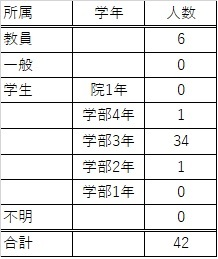
\includegraphics[width=0.\linewidth]{./figure/hyou81.jpg}
\end{center}


\begin{table}[htb]
  \begin{center}
    \caption{評価人数集計}
    \begin{tabular}{|c|c|c|} \hline
      所属 & 学年 & 人数  \\ \hline 
      教員 &  & 6  \\
      一般 &  & 0 \\
      学生 & 院1年 & 0 \\
             & 学部4年 & 1 \\
       & 学部3年 & 34 \\
             & 学部2年 & 1 \\
             & 学部1年 & 0 \\
      合計 &  & 42 \\ \hline
    \end{tabular}
    \label{tab:dist}
  \end{center}
\end{table}
次はそれぞれの評価項目についての平均点を表に記す。
\begin{figure}
\begin{center}
\caption{評価点数集計}
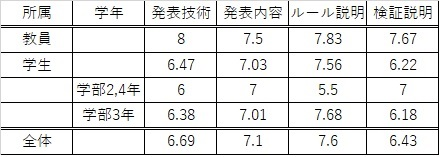
\includegraphics[width=0.5\linewidth]{./figure/hyou82.jpg}
\end{center}
\end{figure}

全体の平均は「発表技術」については6.69、「発表内容」については7.1、「ルール説明」については7.6、「検証説明」については6.43となった。それぞれの項目について高く評価したのは「教員」だった。
次に、それぞれの結果を図\ref{gizyutu}\ref{naiyou}\ref{ru-ru}\ref{kensyou}に示す。

\begin{figure}[h]
 \begin{tabular}{cc}
  \begin{minipage}[h]{0.45\hsize}
  \centering
 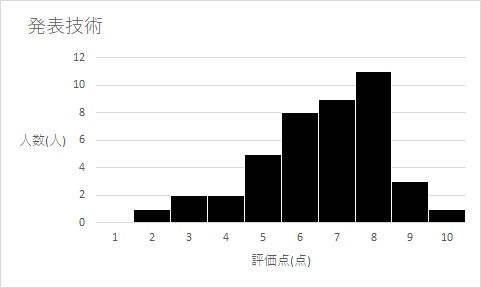
\includegraphics[width=0.7\linewidth]{./figure/gizyutu.jpg}
\caption{発表技術の評価グラフ}
\label{gizyutu}
 \end{minipage} &

\begin{minipage}[h]{0.45\hsize}
  \centering
 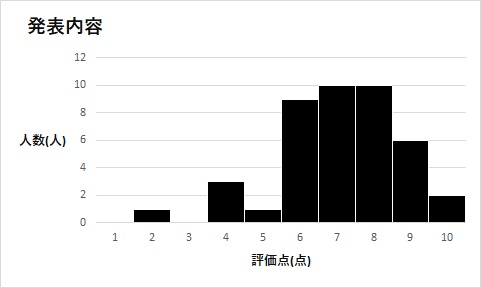
\includegraphics[width=0.7\linewidth]{./figure/naiyou.jpg}
 \caption{発表内容の評価グラフ}
\label{naiyou}
\end{minipage} 
\end{tabular}
\end{figure}

\begin{figure}[h]
 \begin{tabular}{cc}
  \begin{minipage}[h]{0.45\hsize}
  \centering
 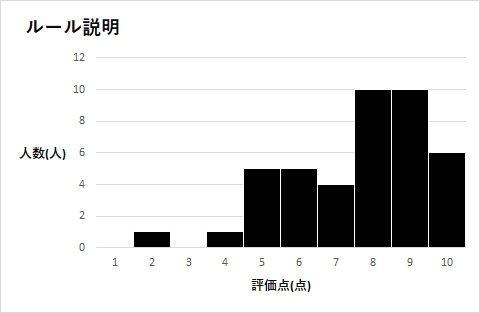
\includegraphics[width=0.7\linewidth]{./figure/ru-ru.jpg}
\caption{ルール説明の評価グラフ}
\label{ru-ru}
 \end{minipage} &

\begin{minipage}[h]{0.45\hsize}
  \centering
 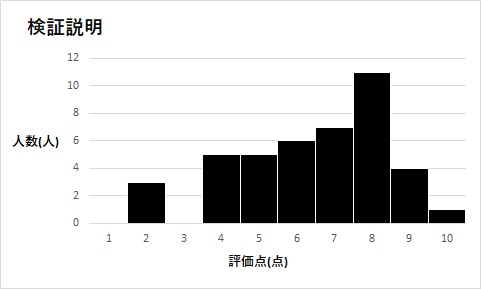
\includegraphics[width=0.7\linewidth]{./figure/kensyou.jpg}
 \caption{検証説明の評価グラフ}
\label{kensyou}
\end{minipage} 
\end{tabular}
\end{figure}
発表技術と発表内容については評価点が共に7,8点と高い評価点が多かった。ルール説明についても同様に高い評価点が多かった、一方で検証説明については4,5点が多い結果となった。

また、「発表技術」と「発表内容」の評点の相関係数は0.71となった。これは、2つの評価項目がかなり関連してると言える数値である。次にコメントについて解析する。
\begin{flushright}
(※文責:葛西隼人)
\end{flushright}

\subsection{コメント解析と改善点}
まず、「発表技術」について、多かったコメントを肯定的なコメントと否定的なコメントに分けて並べる。
肯定的なコメント
\begin{itemize}
\item 複雑な内容をうまく説明してくれた
\item スライド内で図を多様されていて分かりやすかった
\end{itemize}

否定的なコメント
\begin{itemize}
\item 前を見て話してもらえないと聞き取りにくい
\item 説明が少し早い
\end{itemize}

今回はスライドの分量が多く、どうしても早口になってしまったのでこのような意見が多かった。
次に、「発表内容」についても同様に、多かったコメントを肯定的なコメントと否定的なコメントに分けて並べる。
肯定的なコメント
\begin{itemize}
\item 活動内容が明確でよかった
\item 実験・検証が多く、説得力をもたせている
\item 評価基準や比較対象が明確で理解しやすかった
\end{itemize}

否定的なコメント
\begin{itemize}
\item 用語についてより詳しく説明すべき
\item 聞く人の知識が必要になるのでもう少しわかりやすく
\end{itemize}


「発表内容」に関しては、検証の説明があまり理解出来ないとのコメントも見受けられた。最後に重要なアドバイスもいくつかあったため、これについても述べていく。 
\begin{itemize}
\item なぜあのような式を利用することで性能が表されているかの説明がもう少し欲しかった
\item 文字数を減らし簡潔な内容の方がいいと思う
\item 検証結果の魅せ方にもう少し工夫があると良かった(専門的な知識がない人にもわかりやすく)
\end{itemize}
これらの意見に関しても、後期の活動に反映することとする。
以上より中間発表の評価コメントは賛否両論であり、とても参考になった。
\bunseki{※葛西隼人}


\begin{thebibliography}{9}
  \bibitem{pattern1} Christopher M. Bishop(2007) {\it{Pattern Recognition and Machine Learning}} (元田浩 他 訳 (2016) 『パターン認識と機械学習 上』 , 丸善出版)
  \bibitem{basicstrategy} Edward Thorp (1962) {\it{Beat The Dealer:A Winning Strategy for the Game of Twenty One}} (宮崎三瑛(2006)『ディーラーをやっつけろ!』,Vintage)
  \bibitem{complexity} Gregory J. Chaitin(1969)"On the Simplicity and Speed of Programs for Computing Infinite Sets of Natural Numbers",Journal of the Association for Computing Machinery, Vol.16,No.3,July 1969,pp. 407-422
  \bibitem{blakjack2} Roger Baldwin, Wilbert Cantey, Herbert Maisel and James McDermott (1956) "The Optimum Strategy in Blackjack", Journal of the American Statistical Association, 51:275, 419-439
  \bibitem{neuro2} 斎藤康毅 (2016) 『ゼロから作るDeep Learning Pythonで学ぶディープラーニングの理論と実装』, 森北出版株式会社
  \bibitem{blackjack1} 齋藤隆浩 (1999) 『新訂ブラックジャック必勝法』, 株式会社データハウス
  \bibitem{neuro1} 萩原将文 (1994) 『ニューロ・ファジィ・遺伝的アルゴリズム』, 産業図書株式会社
  \bibitem{statistics1} 山内光哉(1987) 『心理・教育のための統計法』, 株式会社サイエンス社
\end{thebibliography}


%暫定削除予定
%\section{ニューラルネットワーク}
\subsection{脳神経回路}
   人間の脳は神経細胞(neuron)とグリア細胞とから成り,情報処理の機能は主に神経細胞が行っているとされる。
  神経細胞は細胞体(soma)と軸索(axon)からなり,神経系を構成する。神経細胞同士のつながりを神経終端(もしくはシナプス)といい
  軸索末端が他の神経細胞の細胞体につながっている形になっている。細胞体と軸索末端との接合部について,
  細胞体側を樹状突起という。軸索末端と樹状突起は厳密に接合しているわけではなく,シナプス間隙と呼ばれる幅$20\sim 50\mathrm{nm}$の空間が
  存在している。また接合部において,軸索側の細胞膜をシナプス前膜(presynaptic cell),樹状突起側の細胞膜をシナプス後膜
  (postsynaptic cell)という。

   神経系を構成する細胞は以上のようになっているが,神経系の動作そのものは電気的な信号である。
  生体において電気現象は,細胞を構成する水溶液中のイオンによって行われる。細胞膜にはイオンポンプという
  イオンを選択的に輸送する機構があり,イオンポンプが能動的にイオンを輸送することで,膜を介した細胞同士で
  イオンが不均等な分布になるように維持される。イオンの不均等な分布は細胞膜を介した電位差を生じさせる。これを
  膜電位(membrane potential)という。膜電位は通常$-60\sim-80\mathrm{mV}$付近であり,この付近の電位を静止電位という。
  細胞は刺激に応じて膜電位を変化させ,この時の一過性の電位を活動電位という。活動電位が軸索末端に達することで
  シナプス前膜からイオンが流入し神経伝達物質という神経細胞における信号伝達を担う物質がシナプス間隙に放出される。
  放出された神経伝達物質をシナプス後膜側の受容体が受け入れることで異なる神経細胞に信号が伝わっていくのである。

   神経伝達物質の放出,吸収によって神経細胞の膜電位は変化する。神経伝達物質の蓄積によって膜電位は徐々に上昇し
  ある閾値に到達すると急激に変化し,その後静止電位に戻り,神経細胞の活性化という。これは神経伝達物質の放出に対応する。

   以上のことをまとめると,まず思考や感情を司る脳は神経細胞による神経系である。神経系の動作は電気信号であり,
  神経伝達物質の輸送によって神経細胞から他の神経細胞に伝わっている。そしてこの輸送は電気信号の過渡的な変化
  によって観測されるということである。
\bunseki{※米村祥裕}

\subsection{単純パーセプトロン}
  神経回路を模倣した演算モデルとして単純パーセプトロンというものが提案された。
  パーセプトロンは入力$\bm{x}=(x_i) \in \mathbb{R}^n $に対して$y=\{0,1\}$を出力する。
  パーセプトロンには入出力値以外に重み(weight)パラメータ$\bm{w}=(w_i) \in \mathbb{R}^n$
  ,閾値$\theta \in \mathbb{R}$がある。入力と出力との関係は式\ref{perceptron}で表される。
  
  \begin{equation}
    \label{perceptron}
    y =
    \left\{
    \begin{aligned}
      0 \quad &\sum_i{w_i x_i} < \theta \\
      1 \quad &\sum_i{w_i x_i} \geq \theta
    \end{aligned}
    \right.
  \end{equation}

  式\ref{perceptron}からわかるように,重みパラメータは入力の伝わりやすさを表している。
  入力値と重みパラメータとの積が閾値以上であれば1,閾値未満であれば0が出力される。
  式\ref{perceptron}は次の式\ref{perceptron2}のように書き直すことができ,この時のパラメータ$b\in \mathbb{R}$をバイアスという。

  \begin{equation}
    \label{perceptron2}
    y =
    \left\{
    \begin{aligned}
      0 \quad &\sum_i{w_i x_i} + b < 0 \\
      1 \quad &\sum_i{w_i x_i} + b \geq 0
    \end{aligned}
    \right.
  \end{equation}

  パーセプトロンによって実際に計算を構築するために,例として2入力AND回路について考えてみる。
  2入力AND回路の真理値表は表1のようになっている。

  \begin{table}[htb]
    \centering
    \caption{AND回路の真理値表}
    \begin{tabular}{|c|c|c|} \hline
      $x_1$ & $x_2$ & $y$ \\ \hline
      0 & 0 & 0 \\ \hline
      0 & 1 & 0 \\ \hline
      1 & 0 & 0 \\ \hline
      1 & 1 & 1 \\ \hline
    \end{tabular}
  \end{table}

  パーセプトロンで2入力AND回路を実現するには,パラメータを式\ref{andperceptronparameter}のように設定すればよい。

  \begin{equation}
    \label{andperceptronparameter}
    \left\{
      \begin{aligned}
        w_1 = 0.7 \\
        w_2 = 0.7 \\
        b = -1.0
      \end{aligned}
    \right.
  \end{equation}

  実際にすべての入力パターンについて重みパラメータと入力値との積の合計を計算してみる。

  \begin{table}[htb]
    \centering
    \caption{パーセプトロンによるAND回路の表現}
    \begin{tabular}{|c|c|c|c|} \hline
      $x_1$ & $x_2$ & $\sum_i{w_i x_i}+b$ & y \\ \hline
      0 & 0 & $-1$ & 0 \\ \hline
      0 & 1 & $-0.3$ & 0 \\ \hline
      1 & 0 & $-0.3$ & 0 \\ \hline
      1 & 1 & 0.4 & 1 \\ \hline
    \end{tabular}
  \end{table}

  同様に2入力OR回路もパラメータ$w_1 = 0.7, w_2 = 0.7, \theta = 0.5$などと設定すれば実現することができる。

  \bunseki{※米村祥裕}
\subsection{多層パーセプトロン}
  単純パーセプトロンでは2入力XOR(排他的論理和)回路は表現することができない。
  そこでパーセプトロンの出力を,他のパーセプトロンの入力とすることを考える。
  XOR回路はAND回路とNOT回路を組み合わせて作ることができるため,パーセプトロンを複数層に
  すれば実現することができる.
  
  \bunseki{※米村祥裕}
\subsection{順伝搬型ニューラルネットワーク}
パーセプトロンでは入力と重みパラメータとの積の総和が閾値以上であれば出力が1,閾値未満であれば0が出力される。
ニューラルネットワークを構成する計算要素(ユニットという)はより一般的に入出力を表現し,式\ref{NN}で表すことができる。

  \begin{equation}
    \label{NN}
    \begin{aligned}
    u ={}^t \bm{wx} + b \\
    y = f(u)
    \end{aligned}
  \end{equation}

  \begin{figure}[htb]
    \begin{center}
      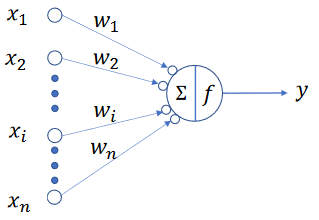
\includegraphics[clip, width=7.0cm]{./figure/neuralnetworkunit.png}
      \caption{ニューラルネットワークのユニット}
    \end{center}
  \end{figure}
  
  式\ref{NN}において$\bm{x} \in \mathbb{R}^n$は入力,$\bm{w} \in \mathbb{R}^n$は重みパラメータである。
  関数$f$を活性化関数という。パーセプトロンはニューラルネットワークの活性化関数にステップ関数を
  用いた特殊な場合であると考えることができる。

  パーセプトロンの場合と同様にニューラルネットワークも複数の層を形成させることができる。
  入力データを受け取る層を入力層,出力データを出力する層を出力層,入力層と出力層との間に存在する
  中間層という。

  \bunseki{※米村祥裕}
\subsection{活性化関数}
活性化関数は用途に応じて使い分けられる。ここでは代表的なものを挙げる。
  \bunseki{※米村祥裕}
\subsubsection{ステップ関数}
ステップ関数は$x\in \mathbb{R}$を入力として$y \in \mathbb{R}$を出力する。関数は式\ref{step_function}
で表される。入力層,中間層で主に使われる。パーセプトロンはステップ関数を利用していると考えることができる。
ステップ関数は連続でない関数であり,出力は0もしくは1である。そのため,後で後述するが,性能向上を考えたときに
関数の表現力に限界があるため,あまり使われなくなっている。

\begin{equation}
  \label{step_function}
  y = \left\{
    \begin{aligned}
      0 \quad x \leq 0 \\
      1 \quad x > 0
    \end{aligned}
  \right.
\end{equation}

\begin{figure}[htb]
  \begin{minipage}{0.5\hsize}
  \begin{center}
    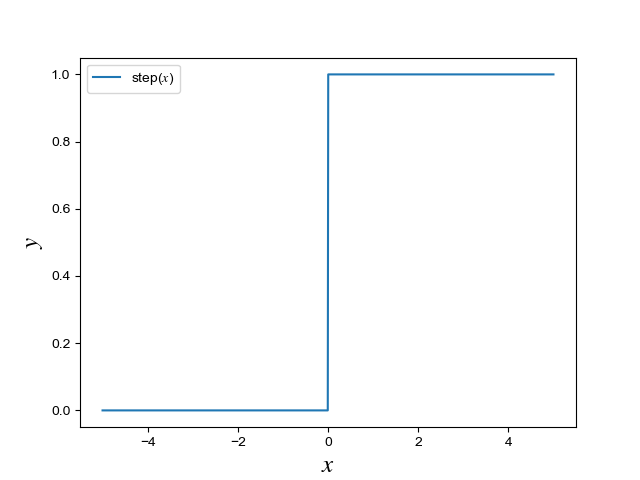
\includegraphics[clip, width=88mm]{./figure/step.png}
    \caption{ステップ関数の概形}
  \end{center}
  \end{minipage}
  \begin{minipage}{0.5\hsize}
  \begin{center}
    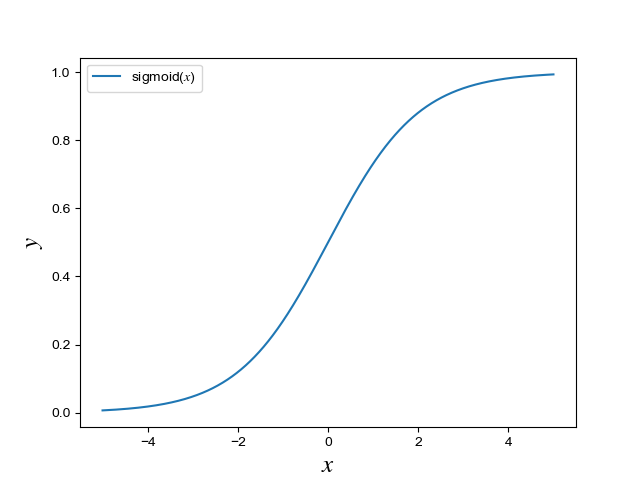
\includegraphics[clip, width=88mm]{./figure/sigmoid.png}
    \caption{シグモイド関数の概形}
  \end{center}
  \end{minipage}
\end{figure}

  \bunseki{※米村祥裕}
\subsubsection{シグモイド関数}
シグモイド関数は$x\in \mathbb{R}$を入力として$y \in \mathbb{R}$を出力する。関数は式\ref{sigmoid_function}で表される。
シグモイド関数はステップ関数とグラフの概形が似ているが,違いとしては連続かつ非線形であるという特徴がある。
また,シグモイド関数の勾配はすべての定義域で0にならない。この性質がニューラルネットワークの性能を向上させるうえで
重要となる。

\begin{equation}
  \label{sigmoid_function}
  y = \frac{1}{1+e^{-x}}
\end{equation}

  \bunseki{※米村祥裕}
\subsubsection{正則化線形関数(ReLU関数)}
正則化線形関数(ReLU)関数は$x\in \mathbb{R}$を入力として$y \in \mathbb{R}$を出力する。関数は式\ref{ReLU_function}で表される。
\begin{equation}
  \label{ReLU_function}
  y = \left\{
    \begin{aligned}
      0 \quad x < 0 \\
      x \quad x \geq 0
    \end{aligned}
  \right.
\end{equation}

  \bunseki{※米村祥裕}
\subsubsection{恒等関数}
恒等関数は出力層で主に用いられる関数である。入力$x\in \mathbb{R}$をそのまま出力として返す。

  \bunseki{※米村祥裕}
\subsubsection{ソフトマックス関数}
ソフトマックス関数は出力層で主に用いられる関数である。特に多クラス分類問題に用いられる。
ソフトマックス関数は$x\in \mathbb{R}^n$を入力として$y \in \mathbb{R}^n$を出力する。入力と出力との関係は次の式\ref{softmax_function}で表される。

\begin{equation}
\label{softmax_function}
y_k = \frac{e^{x_k}}{\sum_i^n e^{x_i}}
\end{equation}

$e^{x_k}$が大きいほど$y$は大きくなる。また$y_k$の総和は1になる。以上の性質を用いて,出力を
対応するクラスである確率であると解釈できる。そのため,$\b{max} \ e^{x_k}$に対応するクラスを出力とすることで,
入力に対していくつかのクラスを分類する問題に適用できる。

\bunseki{※米村祥裕}
%\section{ニューラルネットワークの学習}
本項ではニューラルネットワークの学習について説明する。ニューラルネットワークにおける学習とは教師データから最適なパラメータを自動で設定することを指す。ニューラルネットワークが学習を行うための指標として損失関数というものを導入し、損失関数の値が最も小さくなるようにパラメータを更新することが学習の目的となる。
\begin{flushright}
\bunseki{※伊藤 晋之介}
\end{flushright}

\subsection{損失関数}
損失関数とは、入力データxに対するニューラルネットワークの出力yと教師データtがどの程度一致しているかを表すための指標になるものである。損失関数の値が小さいほどニューラルネットワークの出力と教師データの一致度は高く、逆に損失関数の値が小さいときはニューラルネットワークの出力と教師データの一致度は低いということになる。この損失関数を基準としてニューラルネットワークは各パラメータの値を調整していくことになる。ここでは代表的な損失関数を二つ紹介する。またこれ以降損失関数は\sl{E}と表記する。
\begin{flushright}
\bunseki{※伊藤 晋之介}
\end{flushright}

\subsubsection{最小二乗和誤差}
損失関数でも有名なものの一つに最小二乗和誤差がある。
最小二乗和誤差は次の式で表される。

\begin{equation}
\label{最小二乗和誤差}
E = -\frac{1}{2}\sum_k^n (y_k - t_k)^2
\end{equation}
tは教師データ、yはニューラルネットワークの出力を表す。

$最小二乗和誤差はtとyの差が大きいほど損失関数の値は大きくなり、逆にy=tになるとき損失関数は最小値をとる。$
\begin{flushright}
\bunseki{※伊藤 晋之介}
\end{flushright}

\subsubsection{交差エントロピー誤差}
最小二乗和誤差とは別に交差エントロピー誤差も多く用いられる。交差エントロピー誤差は主に多クラス分類問題で用いられる関数で、出力層の活性化関数ソフトマックス関数とセットで使われる。
交差エントロピー誤差は次の式で表される。

\begin{equation}
\label{交差エントロピー誤差}
E = -\sum_k^n t_k \log y_k
\end{equation}

こちらもyはニューラルネットワークの出力、tは教師データを表す。

\begin{figure}[h]
\begin{center}
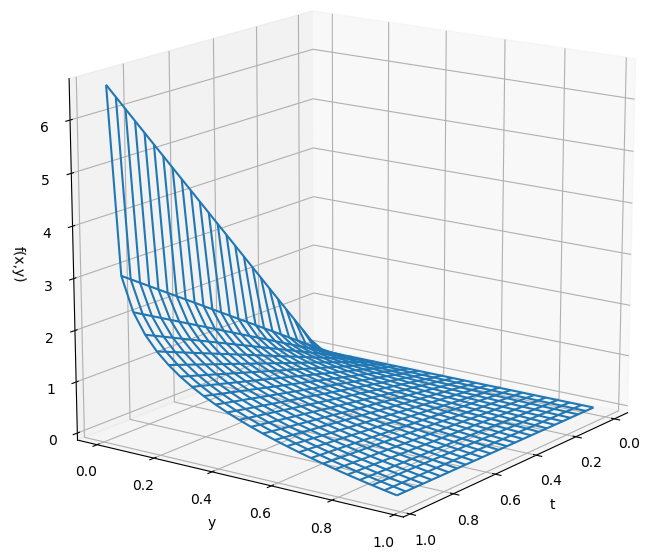
\includegraphics[width=7cm]{./figure./graph2_1.png}
\end{center}
\caption{交差エントロピー誤差1}
\end{figure}

グラフは次のようになるが、ここでtは入力データxが属するクラスの要素のみが1でそれ以外が0という構造をとるものとする。これをone-hot表現という。

\[
  \bm{t} = \left(
    \begin{array}{c}
      1 \\
      0 \\
      0
    \end{array}
	\right)\ or\ 
\bm{t} = \left(
    \begin{array}{c}
      0 \\
      1 \\
      0
    \end{array}
  \right)\ or\ 
\bm{t} = \left(
    \begin{array}{c}
      0 \\
      0 \\
      1
    \end{array}
  \right)
\]

$one-hot表現では教師データはこの3つのどれかで表される。入力データxに対応する出力をy^*とすると、tはxが属するクラスのみ1でそれ以外が0となるため、交差エントロピー誤差の式は次のように変形できる。$

\begin{equation}
\label{交差エントロピー誤差}
E = - \log y^*
\end{equation}
$この時のグラフは図3のようになる。$

\begin{figure}[h]
\begin{center}
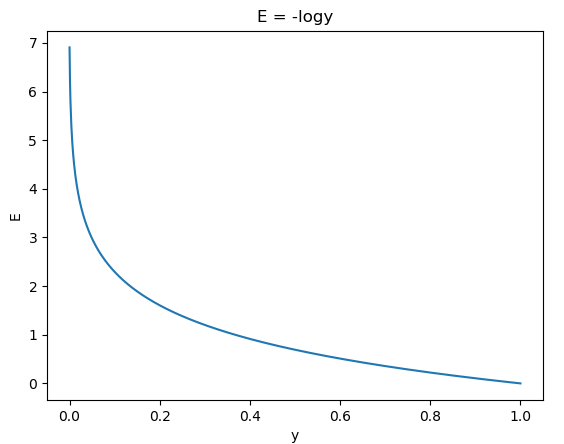
\includegraphics[width=7cm]{./figure./graph2_2.png}
\end{center}
\caption{交差エントロピー誤差2}
\end{figure}

$交差エントロピー誤差はソフトマックス関数と組み合わせて使うことが多いため、y,tはそれぞれ(0\le y \le 1)\ , (0\le t \le 1)となり、確率のように扱える。交差エントロピー誤差はyがtに近い値を出力するほど値が小さくなっていく。交差エントロピー誤差の最小値はy=1、つまりy=tになる時に最小値をとる。またy=0の時は損失関数の値が∞に発散してしまうので、実装する際にはyに微小な値を足し合わせることで発散を防ぐ。$
\begin{flushright}
\bunseki{※伊藤 晋之介}
\end{flushright}

\subsection{パラメータの更新}

ニューラルネットワークのパラメータには次のようなものがある。

\begin{itemize}
\item 重みパラメータ \sl{W}
\item バイアス \sl{b}
\end{itemize}

これらのパラメータを損失関数をもとに更新していく。具体的には損失関数が最小になるようなパラメータを設定していく。しかし一般的には損失関数は複雑であり、ニューラルネットワークのパラメータも層が増えるにつれて数が膨大になっていく。そのため損失関数が最小になる点を求めるのは簡単ではない。そこで損失関数が最小となる点を求めるために用いられる方法の一つに勾配降下法がある。

\begin{flushright}
\bunseki{※伊藤 晋之介}
\end{flushright}

\subsubsection{勾配降下法}
勾配降下法とは関数の最小値を求めるためのアルゴリズムであり、以下の式で表される。
\begin{itemize}
\item{$ある関数がy=f(x)となる時$}
\end{itemize}
\begin{equation}
x_{t+1}=x_t - \eta\frac{\partial f(x_t)}{\partial x}
\end{equation}

$ここで\frac{\partial f(x_t)}{\partial x}はある点x_tでのf(x)の勾配を表す。$
$また\mu は学習率といい、一度の更新でどれだけパラメータを更新するかを決めるものである。この値は大きすぎても小さすぎても学習がうまくいかなくなってしまう。そのため様々な値を試し、適当な大きさに設定していく必要がある。$
具体的な手順は次のようになる。

\begin{enumerate}
\item{ある点xでの関数の勾配を偏微分で求める}
\item{その点から勾配を減らす方向に進む}
\item{上の2つを一定の回数繰り返していく}
\end{enumerate}

$ここでは実際にz=f(x,y)、f(x,y)=x^2+y^2の最小値を勾配法で求めてみる。
x,yの更新式は次のようになる。$
\begin{equation}
x_{t+1} =x_t - \eta \frac{\partial f(x_t,y_t)}{\partial x},\ 
y_{t+1} =y_t - \eta \frac{\partial f(x_t,y_t)}{\partial y}
\end{equation}
$xの初期値x_0=1.7、yの初期値y_0=1.7、学習率\eta = 0.1として勾配法のアルゴリズムを適用すると次のようになる。$

\begin{figure}[h]
\begin{center}
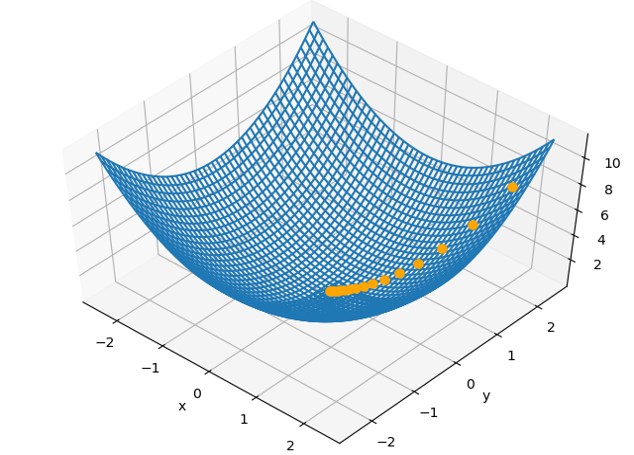
\includegraphics[width=7cm]{./figure./graph3.png}
\end{center}
\caption{勾配降下法の例}
\end{figure}

$f(x,y) = x^2 + y^2の最小値は(x,y)=(0,0)、勾配降下法を用いることで確かに最小値を求めることができることがわかる。$

$ニューラルネットワークの場合の勾配ついて説明していく。ニューラルネットワークの勾配とは重みパラメータに関する損失関数の勾配である。例えば2×3の重みWをもつニューラルネットワークの場合を考える。この時損失関数に対する各重みの勾配\frac{\partial E}{\partial W}は図のようになる。$

\[
  W = \left(
    \begin{array}{ccc}
      W_{11} & W_{12} & W_{13} \\
      W_{21} & W_{22} & W_{23} 
    \end{array}
  \right)
\]

\[
  \frac{\partial E}{\partial W} = \left(
    \begin{array}{ccc}
     \frac{\partial E}{\partial W_{11}} & \frac{\partial E}{\partial W_{12}} & \frac{\partial E}{\partial W_{13}} \\
\\
      \frac{\partial E}{\partial W_{21}} & \frac{\partial E}{\partial W_{22}} & \frac{\partial E}{\partial W_{23}} 
    \end{array}
  \right)
\]
$\frac{\partial E}{\partial W}の各要素はそれぞれの要素の偏微分から構成される。例えば1行目1列目の\frac{\partial E}{\partial W_{11}}はW_{11}の値を変えた場合の数値微分を求めパラメータを更新する。これを各パラメータに対して行う。$

\begin{flushright}
\bunseki{※伊藤 晋之介}
\end{flushright}

\subsection{誤差逆伝播法}
$数値微分でのパラメータの更新は簡単だが計算に時間がかかる。そこでより効率的に計算を行うことができる誤差逆伝播法について説明する。
誤差逆伝播法はニューラルネットワークの出力から損失関数の微分値を入力側へ伝えていく。そうすることで一度の実行で損失関数の各層に対する微分を求めることができるようになる。数値微分と誤差逆伝播法の計算量の違いを比較する。$

数値微分\\
\begin{itemize}
\item{数値微分の場合の計算量はニューラルネットワークのパラメータ量に比例する。}
\item{Nをニューラルネットワークのパラメータ量とする}
\item{$一回の実行にかかる計算量はCN(C:定数)$}
\item{更新するパラメータの数だけ実行する必要がある。}
\item{$最終的な計算量はO(N^2)となる。$}
\end{itemize}

誤差逆伝播法
\begin{itemize}
\item{一度の学習で全てのパラメータを更新することができる。}
\item{パラメータの更新回数はパラメータの量に比例する}
\item{$一度の実行にかかる計算量をCN(C:定数)とする$}
\item{$最終的な計算量はO(N)となる。$}

このため誤差逆伝播法を使うことで効率よくパラメータを更新することができる。
\end{itemize}
\begin{flushright}
\bunseki{※伊藤 晋之介}
\end{flushright}
%\section{パラメータの更新}
{第6章ではニューラルネットワークの学習において重要な役割を果たすパラメータについて学んだ。最適な重みパラメータを探索する最適化手法に始まり、重みパラメータの初期値、ハイパーパラメータの設定方法などである。そこで記されている手法を用いることでニューラルネットワーク(ディープラーニング)の学習を効率的に進めることができ、認識精度を高めることができる。
  \bunseki{※薩田凱斗}
}



\subsection{確率的勾配下降法}
{ニューラルネットワークにおける学習の目的は、損失関数の値をできるだけ小さくするパラーメータを見つけることであり、それを最適化という。最適化は非常に複雑で難解であるためパラメータの勾配を手がかりに探していく。これは確率的勾配下降法と言い非常に単純な最適化の手法である。確率的勾配下降法の数式は以下のように表される。
{
\begin{equation}
\label{eq1}
\bf W \leftarrow W - \eta  \frac{\partial L}{\partial W}
\end{equation}
}
ここで、更新する重みパラメータを{\bf W} 、{\bf W}に関する損失関数の勾配を$\displaystyle \frac{\partial L}{\partial W}$とする。$\displaystyle {\eta}$は学習係数を表し、あらかじめ決めておいた値を使用する。また、式中の$\displaystyle {\leftarrow}$は、右辺の値で左辺の値を更新するということを表している。式(\ref{eq1})で表されるように、確率的勾配下降法は勾配方向へある一定の距離だけ進むという単純な方法であることがわかった。しかし、この確率的勾配下降法には欠点がある。単純で実装も簡単という利点があるが、問題によっては非効率な場合が存在する。その欠点を指摘するために次の関数の最小値を求める問題を考える。
\begin{equation}
\label{eq2}
f(x,y) = \frac{1}{20}x^{2} + y^{2}
\end{equation}
式(\ref{eq2})で表される関数は図\ref{gr1}に示してあるような形状のグラフである。ここで、このグラフで表される関数の勾配を見ていく。
\begin{figure}[H]
\label{gr1}
\centering
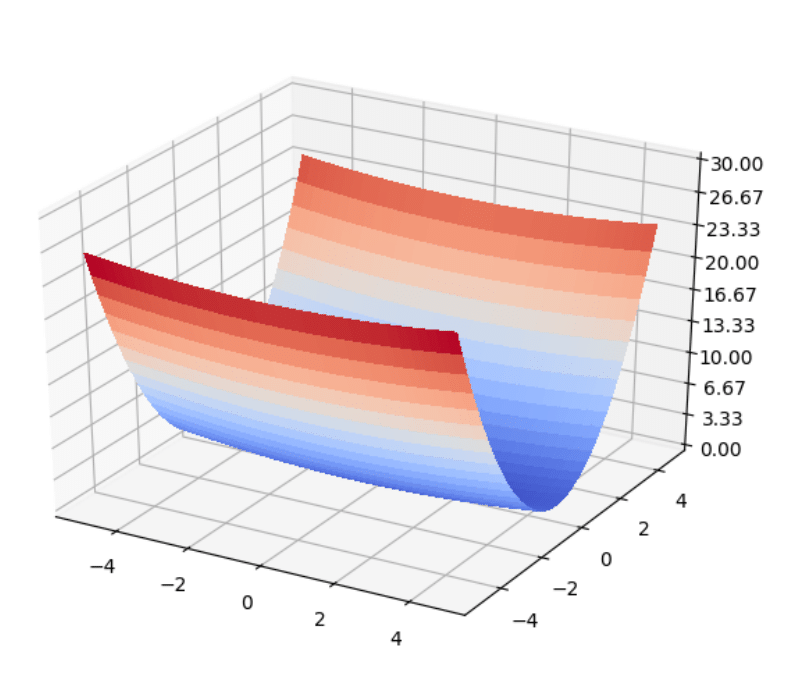
\includegraphics[width=6cm]{./figure/Graph.png}
\caption{$\displaystyle f(x,y) = \frac{1}{20}x^2 + y^2$のグラフ \label{gr1}}
\end{figure} 図1の形状の関数に対して確率的勾配下降法を適応してみる。探索の開始場所である初期値を$\displaystyle (x,y) = (-7.0, 2.0)$から始める。確率的勾配下降法は、図\ref{gr2}に表されるようなジグザグな動きをし、最小値に向かう動きとしてはかなり非効率な経路である。
\begin{figure}[H]
\centering
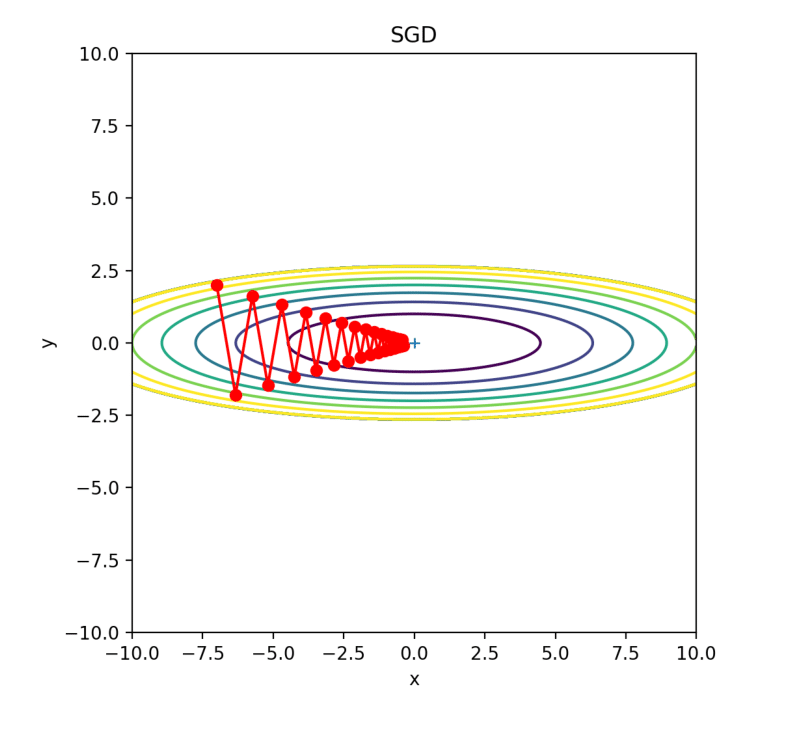
\includegraphics[width=6cm]{./figure/SGD.png}
\caption{SGDによる最適化の更新経路 \label{gr2}}
\end{figure}つまり、確率的勾配下降法の欠点は、関数の形状が等方的出ないと、非効率な経路で探索することになる点にあることがわかる。確率的勾配下降法の非効率な最小値探索経路の原因は、勾配の方向が本来の最小値ではない子方向を指していることにある。そこで、確率的勾配下降法のように単に勾配方向へ進むよりも、より優れた探索方法が求められる。この確率的勾配下降法の欠点を改善するために、Momentum、AdaGrad、Adamという3つの最適化手法を学んだ。
\begin{flushright}
  (※文責:薩田凱斗)
\end{flushright}

}




\subsection{Momentum}
{Momentumは「運動量」という意味の言葉であり、以下のような数式で表される。
\begin{equation}
\label{eq3}
\bf v \leftarrow \alpha v - \eta  \frac{\partial L}{\partial W}
\end{equation}

\begin{equation}
\label{eq4}
\bf W \leftarrow W + v
\end{equation}確率的勾配下降法と同じく、{\bf W}は更新する重みパラメータ、$\displaystyle \frac{\partial L}{\partial W}$は{\bf W}に関する損失関数の勾配、$\displaystyle {\eta}$は学習係数を表す。そして、{\bf v}という変数は速度を表す。式(\ref{eq3})では、物体が勾配方向に力を受け、その力によって物体の速度が加算されるという物理法則を表している。Momentumはボールが地面を転がるような動きに似ている。また、式(\ref{eq3})では、$\displaystyle {\alpha} \bf v$という項があるが、それは物体が何も力を受けないときに徐々に減速するための役割を担っている。物理では、地面の摩擦や空気抵抗に対応する。図\ref{gr3}はMomentumを用いて式(\ref{eq2})の最適化問題を解いた結果である。確率的勾配下降法との大きな違いは、滑らかに最小値に向かっていることである。これは、$\displaystyle x$軸方向に受ける力はとても小さいが、常に同じ方向の力を受けるため、同じ方向へ一定して加速することになる。反対に、$\displaystyle y$軸方向には受ける力は大きいが、正と負の方向の力を交互に受けるため、それらが互いに打ち消し合い、$\displaystyle y$軸方向の速度は安定しない。それゆえ、確率的勾配下降法と比べ、$\displaystyle x$軸方向へと早く近ずくことができ、より滑らかに向かうことができる。
\begin{figure}[H]
\centering
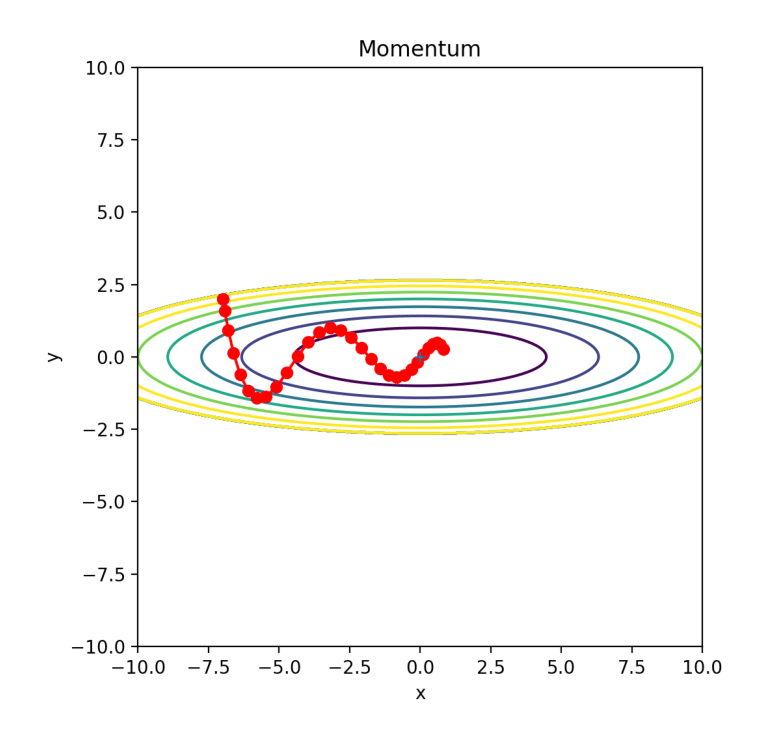
\includegraphics[width=6cm]{./figure/Momentum.png}
\caption{Momentumによる最適化の更新経路 \label{gr3}}
\end{figure}
\begin{flushright}
  (※文責:薩田凱斗)
\end{flushright}
}






\subsection{AdaGrad}
{ニューラルネットワーク の学習では学習係数$\displaystyle {\eta}$の値が重要になる。学習係数が小さすぎると学習に時間がかかりすぎてしまい、逆に大きすぎると発散して正しい学習が行えない。そこで、学習係数に関する有効な方法の1つに学習係数の減衰というものがある。最初に大きく学習し、徐々に小さく学習するというものである。学習係数を徐々に下げていくという考えは、パラメータ全体の学習係数の値を一括して下げることに担当します。これらをさらに発展させたものがAdaGradである。1つ1つのパラメータに対して独自の値を設定する。AdaGradはパラメータの要素ごとに適応的に学習係数を調整しながら学習を行う手法であり、以下のような数式で表される。
\begin{equation} 
\label{eq5}
\bf h \leftarrow  h + \frac{\partial L}{\partial W} \bigodot \frac{\partial L}{\partial W}
\end{equation}

\begin{equation}
\label{eq6}
\bf W \leftarrow W - \eta \frac{1}{\sqrt h}  \frac{\partial L}{\partial W}
\end{equation}確率的勾配下降法と同様に、{\bf W}は更新する重みパラメータ、$\displaystyle \frac{\partial L}{\partial W}$は{\bf W}に関する損失関数の勾配、$\displaystyle {\eta}$は学習係数を表す。ここでは、{\bf h}という変数は式(\ref{eq5})で示されるように、これまでに経験した勾配の値を2乗和として保持する。また、式(\ref{eq5})の$\displaystyle {\bigodot}$は行列の要素ごとの掛け算を意味する。そして、パラメータ更新の際に$\displaystyle \frac{1}{\sqrt h}$を蒸散することで、学習のスケールを調整する。これは、パラメータの要素のなかで大きく更新された要素は、学習係数が小さくなることを意味する。つまり、よく働いたパラメータの学習係数は次第に小さくなるという学習係数の減衰を、パラメータの要素ごとに行うことができる。図\ref{gr4}は、AgaGradを用いて式(\ref{eq2})の最適化問題を解いた結果のグラフである。
\begin{figure}[H]
\centering
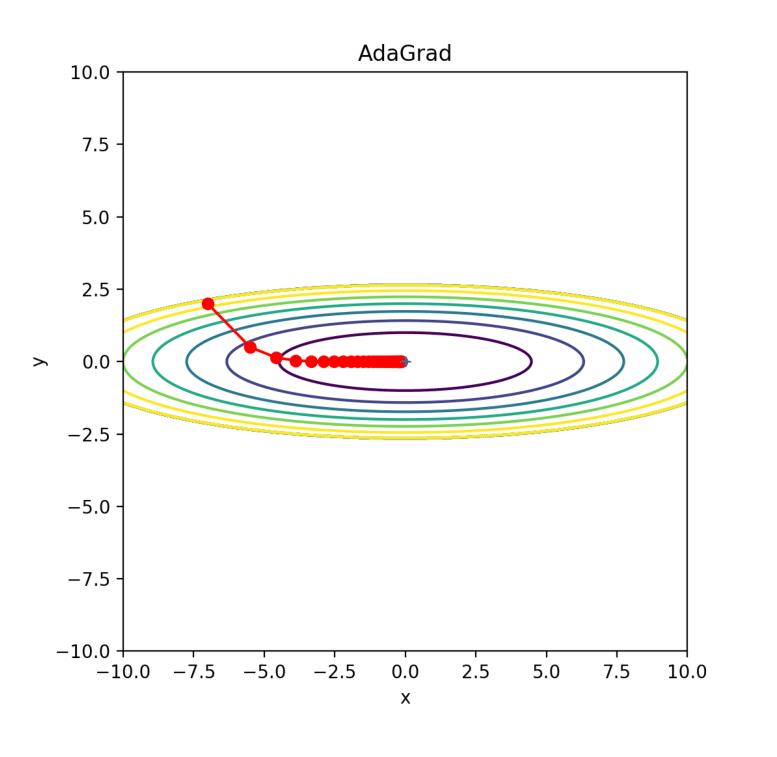
\includegraphics[width=6cm]{./figure/AdaGrad.png}
\caption{AdaGradによる最適化の更新経路 \label{gr4}}
\end{figure}
この結果を見ると、最小値に向かって効率的に動いているのがわかる。$\displaystyle y$軸方向へは勾配が大きいため、最初は大きく動く。その動きに比例し、更新のステップが小さくなるように調整が行われる。そのため、$\displaystyle y$軸方向への更新度合いは弱められていき、滑らかな動きになる。
\begin{flushright}
  (※文責:薩田凱斗)
\end{flushright}
}






\subsection{Adam}
{Adamとは、MomentumとAdaGradを融合した手法であり2015年に提案された新しい手法である。その理論はやや複雑であるが、直感的にはMomentumとAdaGradを融合させ、両者の利点を組み合わせたような探索手法である。この2つの手法を組み合わせることにより、効率的にパラメータ空間を探索することが期待できる。また、ハイパーパラメータのバイアス補正が行われていることもAdamの特徴である。図\ref{gr5}はAdamを用いて式(\ref{eq2})の最適化問題を解いた結果のグラフである。
\begin{figure}[H]
\centering
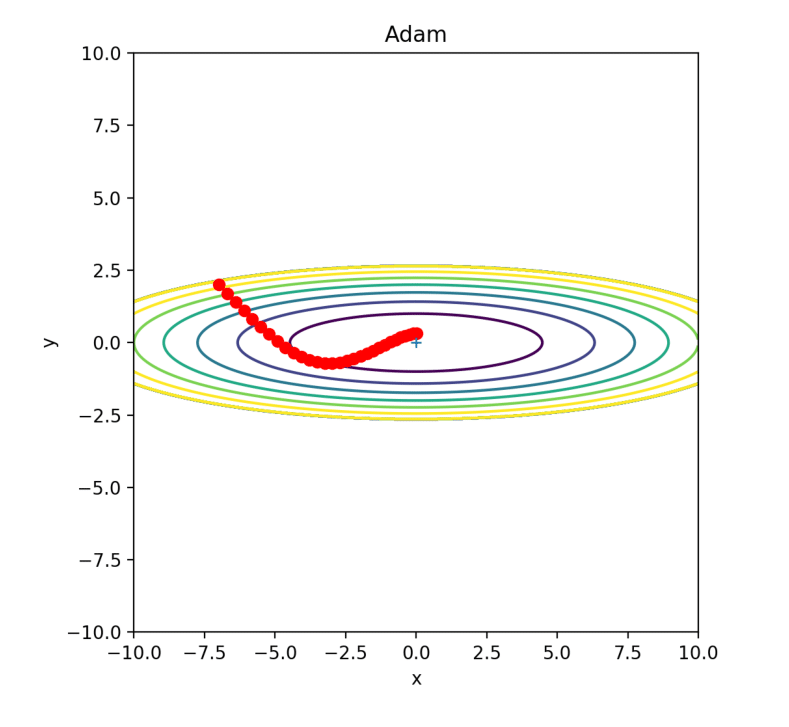
\includegraphics[width=6cm]{./figure/Adam.png}
\caption{Adamによる最適化の更新経路 \label{gr5}}
\end{figure}
図\ref{gr5}で示すように、Adamによる更新の過程は、ボールが転がるような動きをしている。Momentumとも似たような動きをしているが、Momentumよりも左右の揺れが軽減されているのがわかる。これは、学習の更新度合いが適応的に調整されることによってもたらされる。
\begin{flushright}
  (※文責:薩田凱斗)
\end{flushright}
}



\subsection{比較}
{SGD、Momentum、AdaGrad、Adamの4種類のパラメータ更新手法を見てきたわけだが、それぞれに特徴があり、解く問題によって結果が変わってくるので得意な問題、不得意な問題がある。また、ハイパーパラメータ(学習係数)つまり、この手法が最も良い更新手法であるとは一概には言えない。多くの研究ではSGDが今でも使われている。どの手法がより適応しているかを試すためにMomentumやAdaGrad、Adamなども使用してみる価値がある。
\begin{flushright}
  (※文責:薩田凱斗)
\end{flushright}
}

%\section{遺伝的アルゴリズム}
\subsection{生物進化メカニズムの概要}

遺伝的アルゴリズムは進化計算とも呼ばれる,生物の進化メカニズムを応用した
近似最適化アルゴリズムである。環境に適応している生物は生存しつつ増殖する。
増殖には,生物自身の情報を保有している遺伝子が介在している。

単細胞生物をはじめとする下等生物は主に体細胞分裂を行うことで増殖する。体細胞分裂(または無性生殖)では
生物が持つ自信の設計情報,すなわち遺伝子が保有する情報は分裂した後の個体と前の個体とで
完全に一致する。

一方で人間を含む高等生物では,主に有性生殖によって増殖する。体細胞分裂は単一の個体で行われる
のに対して,有性生殖では2つの個体によって行われる。有性生殖を行う2個体の両方の遺伝子から
新たに誕生する個体の遺伝子が再生成され,親個体と子個体とで違った遺伝情報を保持するようになる。

以上の無性生殖,有性生殖による遺伝情報の伝達以外にも個体の遺伝情報を変化させ得る要因が存在する。
生物個体の完全なコピーを作る場合でも,有性生殖によって遺伝子を組み合わせる場合でも,遺伝子の複写
作業は物理的な空間で行われるため,化学的な要因や放射線による破壊等で遺伝情報が元の個体生成プロセス
とは別に変化することがある。これを突然変異という。突然変異は生殖時のエラーとも言えるが,生物の進化においては
重要な要素の一つとなっている。

増殖の過程は大まかに以上のような過程で親個体から子個体が発生するが,もう一つの重要な要素が自然淘汰である。
どの個体も同じように生存し,子孫を残すわけではなく,環境に適応できない個体および遺伝形質は長い時間をかけて
淘汰される。結果として比較的環境に適応している個体群,遺伝形質が存続するようになる。これを自然淘汰という。

遺伝的アルゴリズムは自然界に存在する生殖のメカニズム,自然淘汰のメカニズムを計算に応用した
アルゴリズムである。

  \bunseki{※米村祥裕}
\subsection{遺伝子の構造}
生物の遺伝情報はDNAによって保持され,DNAは主に4種類の塩基によって構成される。
DNAは塩基の並び方によって遺伝情報を表現する。一つの遺伝子座(塩基配列上の位置)における
遺伝子の組み合わせを遺伝子型(genotype)という。ある遺伝子によってほぼ決定される形質のことを
遺伝子の表現型(phenotype)という。表現型は厳密に遺伝子によってのみ決定されるわけではなく,
他の遺伝子,環境などによっても変化しうる。

  \bunseki{※米村祥裕}
\subsection{単純遺伝的アルゴリズム}
前節までで説明した進化メカニズムを基にして,考案されたのが単純遺伝的アルゴリズム(Simple Genetic Algorithm)である。
単純遺伝的アルゴリズムは主に次の処理からなる。

\begin{itemize}
  \item 符号化(遺伝子型の決定,コーディングという)
  \item 環境(問題の要件)に対する適応度の算出
  \item 選択(Selection)
  \item 交叉(Cross Over)
  \item 突然変異(Mutation)
\end{itemize}

  \bunseki{※米村祥裕}
\subsubsection{符号化}
遺伝子の構造については先に説明したように,遺伝子座上の4種類の塩基の並びによって情報が記述される。
単純遺伝的アルゴリズムの場合も同様に,対象とする問題を2進ビット列に置き換える。まずそれぞれの遺伝子座を
表現型と対応させる必要がある。表現型は例えば,特定の文字列の生成にアルゴリズムを適用する場合は文字に相当する。
例として英字アルファベットからなる特定の文字列を単純遺伝的アルゴリズムで生成する場合は,文字をビット列に置き換える。
英字アルファベットは26文字であるから2進数表現にした場合に必要なビット数は1文字あたり5ビットとなる。さらに文字列長を$\b{n}$とすると
遺伝子座数は$n$個となるので,1個体を表現するのに必要な情報量は$5\b{n}$ビットとなる。

  \bunseki{※米村祥裕}
\subsubsection{適応度の算出}
生成された個体が問題に対してどの程度適応しているかを算出するために,まずは個体の遺伝情報,すなわち符号化によって
得られたビット列を表現型に変換する。符号化の項目で挙げた文字列生成の例では,文字列を構成する英字アルファベット1文字当たり
5ビットとなっているので,ビット列全体を5ビットずつに分け,分けた5ビットごとに英字アルファベットに変換する。
そして,一致している要素の個数等で問題の解により近い個体の適応度が高くなるように計算を行う。

適応度の算出は,アルゴリズムを適用する問題に応じて異なる。

  \bunseki{※米村祥裕}
\subsubsection{選択}
複数の個体からなる集団から相対的により良い個体を次世代に残すことでより最適な解に近づける。
基本的には適応度が高い個体が残りやすいように選択を行う。選択のアルゴリズムとしてはルーレット法(適応度比例選択)や
トーナメント法,エリート選択法,ランキング法等が用いられる。

  \bunseki{※米村祥裕}
\subsubsection{ルーレット法(適応度比例選択)}
集団$P$中のある個体$i$が選択される確率$p_i$を個体$i$の適応度$f_i$を基に式で算出される。

\begin{equation}
  p_i = \frac{f_i}{\sum_{j\in P} f_j}
\end{equation}

適応度に比例して選択される確率が増加するため,適応度比例選択と呼ばれる。

  \bunseki{※米村祥裕}
\subsection{交叉}
交叉は有性生殖における,遺伝情報の交換に相当する処理である。
交叉のアルゴリズムとしては一点交叉,二点交叉や一様交叉などが提案されている。

  \bunseki{※米村祥裕}
\subsubsection{一点交叉}
2つの個体を表すビット列をそれぞれ$s_1$,$s_2$とする。交叉を行う点をビット列中から
選択する。交叉を行う点以降のビット列について,$s_1$,と$s_2$とで交換する。これを一点交叉という。

  \bunseki{※米村祥裕}
\subsubsection{二点交叉}
一点交叉の場合は交叉を行う点を1箇所選んだが,二点交叉では2箇所選ぶ。選ばれた2点の間の
ビット列を交換する。

  \bunseki{※米村祥裕}
\subsubsection{一様交叉}
一様交叉ではまず遺伝子を表すビット列と同じ長さのビット列をランダムに生成する。
この時ランダムに生成されたビット列をマスクと呼ぶことにし,$i$番目のビットを$t_i \in {0, 1}$と表す。
$t_i = 1$であれば,二つの個体を表すそれぞれのビット列の$i$番目の要素を交換する。
$t_i = 0$であれば,交換を行わない。

一様交叉において$t_i$の内容によってどのように処理を行うかは実装によって異なることがある。

  \bunseki{※米村祥裕}
\subsubsection{突然変異}
交叉のみでは個体群の変化が小さく,局所的な解に陥ってしまうことがある。そのため,強引に異なる個体を生成する必要があり,
遺伝的アルゴリズムでは突然変異という処理によってこれを行う。具体的には,各個体の各ビット列上のビットに対して,一定の確率で
値を反転させる。これによってビット列の状態が確率的に変化する。

  \bunseki{※米村祥裕}


\end{document}
